\documentclass{beamer}
\usetheme{Frankfurt}
\usepackage[utf8]{inputenc}
\usepackage{charter}
\usepackage{graphicx}
\usepackage{amsmath}
\usepackage{amssymb}
\usepackage{listings}
\usepackage{animate}
\usepackage{bm}
\usepackage{mathtools}
\usepackage{physics}
\usepackage{caption}
\usepackage{tikz}
\usepackage{tikz-cd}
\captionsetup[figure]{labelformat=empty}
\mathtoolsset{showonlyrefs}
\beamertemplatenavigationsymbolsempty

\let\vec\bm

\usepackage{tikzit}
\documentclass{beamer}
\usetheme{Frankfurt}
\usepackage[utf8]{inputenc}
\usepackage{charter}
\usepackage{graphicx}
\usepackage{amsmath}
\usepackage{amssymb}
\usepackage{listings}
\usepackage{animate}
\usepackage{bm}
\usepackage{mathtools}
\usepackage{physics}
\usepackage{caption}
\usepackage{tikz}
\usepackage{tikz-cd}
\captionsetup[figure]{labelformat=empty}
\mathtoolsset{showonlyrefs}
\beamertemplatenavigationsymbolsempty

\let\vec\bm

\usepackage{tikzit}
\documentclass{beamer}
\usetheme{Frankfurt}
\usepackage[utf8]{inputenc}
\usepackage{charter}
\usepackage{graphicx}
\usepackage{amsmath}
\usepackage{amssymb}
\usepackage{listings}
\usepackage{animate}
\usepackage{bm}
\usepackage{mathtools}
\usepackage{physics}
\usepackage{caption}
\usepackage{tikz}
\usepackage{tikz-cd}
\captionsetup[figure]{labelformat=empty}
\mathtoolsset{showonlyrefs}
\beamertemplatenavigationsymbolsempty

\let\vec\bm

\usepackage{tikzit}
\documentclass{beamer}
\usetheme{Frankfurt}
\usepackage[utf8]{inputenc}
\usepackage{charter}
\usepackage{graphicx}
\usepackage{amsmath}
\usepackage{amssymb}
\usepackage{listings}
\usepackage{animate}
\usepackage{bm}
\usepackage{mathtools}
\usepackage{physics}
\usepackage{caption}
\usepackage{tikz}
\usepackage{tikz-cd}
\captionsetup[figure]{labelformat=empty}
\mathtoolsset{showonlyrefs}
\beamertemplatenavigationsymbolsempty

\let\vec\bm

\usepackage{tikzit}
\input{main.tikzstyles}

\pgfdeclareimage[width=\paperwidth]{titlebackground}{Images/title-slide-background.png}
\setbeamerfont{subtitle}{size=\tiny}
\setbeamertemplate{endpage}{
	\begin{picture}(0,0)
		\scalebox{1.01}{
		\put(-28.5,-163){%
			\pgfuseimage{titlebackground}
		}
		}
		\put(0,-115){%
			\begin{minipage}[b][4.5cm][t]{0.5\textwidth}
				\color{white}
				\usebeamerfont{title}
				{\textbf{Thank Your} \\ \textbf{For You Attention !}}
			\end{minipage}
		}
	\end{picture}
}
\setbeamertemplate{title page}{
	\begin{picture}(0,0)
		\scalebox{1.01}{
			\put(-28.5,-163){%
				\pgfuseimage{titlebackground}
			}
		}
		\put(0,-60){%
			\begin{minipage}[b][4.5cm][t]{0.7\textwidth}
				\color{white}
				\usebeamerfont{title}
				{\inserttitle\\[0.9cm]}
				\usebeamerfont{subtitle}
				{\insertauthor\par}
				{\insertinstitute\\[0.3cm]}
				{\insertdate}
			\end{minipage}
		}
	\end{picture}
}


%% General slide formatting %%

\definecolor{oxfordblue}{RGB}{4,30,66}
\definecolor{oxfordred}{RGB}{207,48,42}

\pgfdeclareimage[width=0.9cm]{oxfordlogo}{Images/oxford-logo.png}
\pgfdeclareimage[width=1cm]{mathslogo}{Images/mathematics-logo.png}
\pgfdeclareimage[width=1.2cm]{ngslogo}{Images/ngs-logo.png}
\pgfdeclareimage[width=1.2cm]{petsclogo}{Images/petsc-logo.png}
\pgfdeclareimage[width=1.2cm]{firedrakelogo}{Images/firedrake-logo.png}

\setbeamertemplate{headline}
{%
	\begin{picture}(0,0)
		\put(314,-50){%
			\pgfuseimage{oxfordlogo}
		}
		\put(20,-55){%
			\rule{320pt}{0.4pt}
		}
	\end{picture}
}
\def\ngshead{
	\begin{picture}(0,0)
		\put(278,0){%
			\pgfuseimage{ngslogo}
		}
		\put(-8,-5){%
			\rule{325pt}{0.4pt}
		}
	\end{picture}
}
\def\petschead{
	\begin{picture}(0,0)
		\put(278,0){%
			\pgfuseimage{petsclogo}
		}
		\put(-8,-5){%
			\rule{325pt}{0.4pt}
		}
	\end{picture}
}
\def\firedrakehead{
	\begin{picture}(0,0)
		\put(278,0){%
			\pgfuseimage{firedrakelogo}
		}
		\put(-8,-5){%
			\rule{325pt}{0.4pt}
		}
	\end{picture}
}
\setbeamertemplate{frametitle}
{%
	\begin{picture}(0,0)
		\put(-8,-20){%
			\normalsize\textbf{\color{oxfordblue}\insertframetitle}
		}
		\put(-8,-32){%
			\normalsize\textbf{\color{oxfordblue}\insertframesubtitle}
		}
	\end{picture}
}

\setbeamertemplate{footline}
{%
	\begin{picture}(0,0)
		\put(20,30){%
			\rule{320pt}{0.4pt}
		}
		\put(20,14){%
			\pgfuseimage{mathslogo}
		}
		\put(100,14){%
			\color{oxfordblue}\insertshortdate
		}
		\put(160,14){%
			\color{oxfordblue}\insertshorttitle
		}
		\put(337,14){%
			\color{oxfordblue}\insertframenumber
		}
	\end{picture}%
}
\def\footer{
	\begin{picture}(0,0)
		\put(-308,-75){%
			\rule{325pt}{0.4pt}
		}
		\put(-308,-91){%
			\pgfuseimage{mathslogo}
		}
		\put(-228,-91){%
			\color{oxfordblue}\tiny\insertshortdate
		}
		\put(-168,-91){%
			\color{oxfordblue}\tiny\insertshorttitle
		}
		\put(9,-91){%
			\color{oxfordblue}\tiny\insertframenumber
		}
	\end{picture}
}

\setbeamercolor{block title}{bg=oxfordblue!30,fg=black}
\setbeamercolor{palette primary}{bg=oxfordblue,fg=white}

\definecolor{codegreen}{rgb}{0,0.6,0}
\definecolor{codegray}{rgb}{0.5,0.5,0.5}
\definecolor{codepurple}{rgb}{0.58,0,0.82}
\definecolor{backcolour}{rgb}{0.95,0.95,0.92}

\lstdefinestyle{mystyle}{
	%backgroundcolor=\color{backcolour},   
	commentstyle=\color{codegray},
	keywordstyle=\color{oxfordblue},
	numberstyle=\tiny\color{codegray},
	stringstyle=\color{codegreen},
	basicstyle=\ttfamily\footnotesize,
	breakatwhitespace=false,         
	breaklines=true,                 
	captionpos=b,                    
	keepspaces=true,                 
	numbers=left,                    
	numbersep=5pt,                  
	showspaces=false,                
	showstringspaces=false,
	showtabs=false,                  
	tabsize=2
}
\AtBeginSection[]{
  \begin{frame}
  \vfill
  \centering
  \begin{beamercolorbox}[sep=8pt,center,shadow=true,rounded=true]{title}
    \usebeamerfont{title}\insertsectionhead\par%
  \end{beamercolorbox}
  \vfill
  \end{frame}
}

\lstset{style=mystyle}

%% Information (author, title, etc.) %%
\title[ngsPETSc]{ngsPETSc: NETGEN meets PETSc} % short title for footer
\author%
{%
	\sc{P.~E.~Farrell}*, \sc{S.~Zampini$\dag$}, \underline{\sc{U.~Zerbinati}}*\\
}
\institute%
{%
	* \textit{Mathematical Institute}\\
	\;\textit{University of Oxford}\\
	$\newline$
	$\dag$ \textit{Extreme Computing Research Center}\\
	\;\textit{King Abdullah University of Science and Technology}\\	
}

\date[\textbf{DD28}]{28 International Conference on Domain Decomposition Methods, 29th Jannuary 2024, KAUST} % short date for footer



%% Content of slides %%

\begin{document}
	\begin{frame}[plain]
		\titlepage
	\end{frame}
	\begin{frame}[plain]
		\frametitle{NETGEN}
		\ngshead
		$\newline$
		$\newline$
		NETGEN is an advancing front 2D/3D-mesh generator, with many interesting features.
		$\newline$
		$\newline$
		\begin{minipage}{0.58\textwidth}
			\begin{itemize}
				\item[\color{oxfordblue}$\blacktriangleright$] The geometry we intend to mesh can be described by \textbf{Constructive Solid Geometry} (CSG), in particular we can use \textbf{Opencascade} to describe our geometry.
				\item[\color{oxfordblue}$\blacktriangleright$] It is able to construct isoparametric meshes, which conform to the geometry.
			\end{itemize}
		\end{minipage}
		\qquad
		\begin{minipage}{0.3\textwidth}
			\begin{figure}
				\centering
				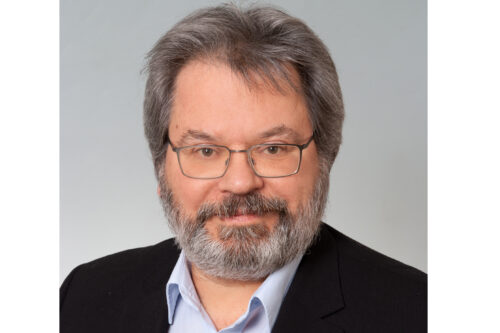
\includegraphics[scale=1.]{Figures/Schoeberl.jpg}
				\begin{center}
					\qquad\small Joachim Sc\"{o}berl
				\end{center}
			\end{figure}
			\vspace{0.3cm}
		\end{minipage}
	\end{frame}

	\begin{frame}[plain]
		$\newline$ 
		$\newline$ 
		\frametitle{PETSc}
		\petschead
		$\newline$
		$\newline$ 
		PETSc stands for Portable, Extensible Toolkit for Scientific Computation, is a library for the scalable (parallel) solution of scientific applications modeled by partial differential equations (PDEs).
		$\newline$
		\begin{minipage}{0.58\textwidth}
			\begin{itemize}
				\item[\color{oxfordblue}$\blacktriangleright$] \textbf{PETSc KSP} provides access to extremly efficent Krylov solvers.
				\item[\color{oxfordblue}$\blacktriangleright$] \textbf{PETSc SNES} provides access to extremly efficent non-linear solvers, with line-searching and trust region capabilities.
			\end{itemize}
		\end{minipage}
		\qquad
		\begin{minipage}{0.3\textwidth}
			\begin{figure}
				\centering
				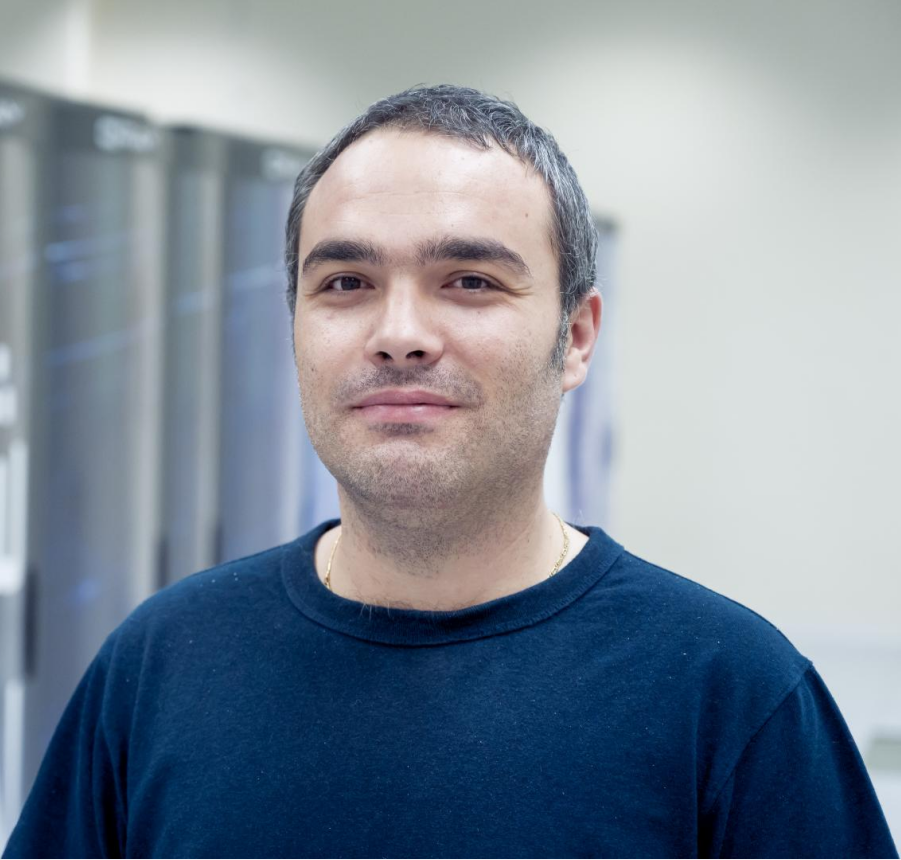
\includegraphics[scale=0.15]{Figures/Zampini.png}
				\begin{center}
					\;\;\small Stefano Zampini
				\end{center}
			\end{figure}
		\end{minipage}
		\vspace{3cm}
	\end{frame}
	\begin{frame}
		\frametitle{ngsPETSc -- NETGEN/NGSolve}
		$\newline$
		\textbf{ngsPETSc} is an interface between NETGEN/NGSolve and \textbf{PETSc}. In particular, \textbf{ngsPETSc} provides new capabilities to \textbf{NETGEN}/\textbf{NGSolve} such as:
		$\newline$
		\begin{itemize}
			\item[\color{oxfordblue}$\blacktriangleright$] Access to all linear solver capabilities of \textbf{KSP}.
			\item[\color{oxfordblue}$\blacktriangleright$] Access to all preconditioning capabilities of \textbf{PC}.
			\item[\color{oxfordblue}$\blacktriangleright$] Access to all non-linear solver capabilities of \textbf{SNES}.
			\item[\color{oxfordblue}$\blacktriangleright$] Access to all mesh refinement capabilities of \textbf{DMPLEX}.
		\end{itemize}
	\end{frame}
	\begin{frame}[plain]
		$\newline$ 
		\petschead
		\frametitle{PETSc DMPlex}
		$\newline$ 
		$\newline$
		\begin{minipage}{0.58\textwidth}
			\textbf{PETSc DMPlex} handles unstructured grids using the generic \textbf{PETSc} interface for hierarchy and multi-physics. 
			$\newline$
			\begin{itemize}
				\item[\color{oxfordblue}$\blacktriangleright$] \textbf{PETSc DMPlex} provides a wide variety of primitive mesh operations such as: \textit{meet}, \textit{clousre}, \textit{cone}, etc
				\item[\color{oxfordblue}$\blacktriangleright$] \textbf{PETSc DMPlex} provides a wide variety of mesh refinement operations such as: \textit{unifrom refinement}, \textit{Alfeld refinement}, \textit{box refinement}, etc
			\end{itemize}
		\end{minipage}
		\qquad
		\begin{minipage}{0.33\textwidth}
			\begin{figure}
				\centering
				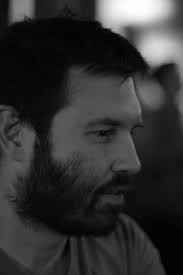
\includegraphics[scale=0.5]{Figures/Kneply.jpeg}
				\begin{center}
					\hspace{0.5cm}\small Matthew G.~Knepley
				\end{center}
			\end{figure}
		\end{minipage}
	\end{frame}
	\begin{frame}[plain]
		\firedrakehead
		$\newline$
		$\newline$
		\textbf{Firedrake} is an automated system for the solution of partial differential equations using the finite element method (FEM).
		$\newline$
		$\newline$
		\begin{minipage}{0.58\textwidth}
			\begin{itemize}
				\item[\color{oxfordblue}$\blacktriangleright$] Variational formulation can be easily defined using the \textbf{UFL} language.
				\item[\color{oxfordblue}$\blacktriangleright$] Wide class of finite elements are available, including $H(div)$, $H(curl)$, $H^1$ and $H^2$.
				\item[\color{oxfordblue}$\blacktriangleright$] Provides access to \textbf{PETSc} linear solvers and non-linear solvers.
			\end{itemize}
		\end{minipage}
		\qquad
		\begin{minipage}{0.3\textwidth}
			\begin{figure}
				\centering
				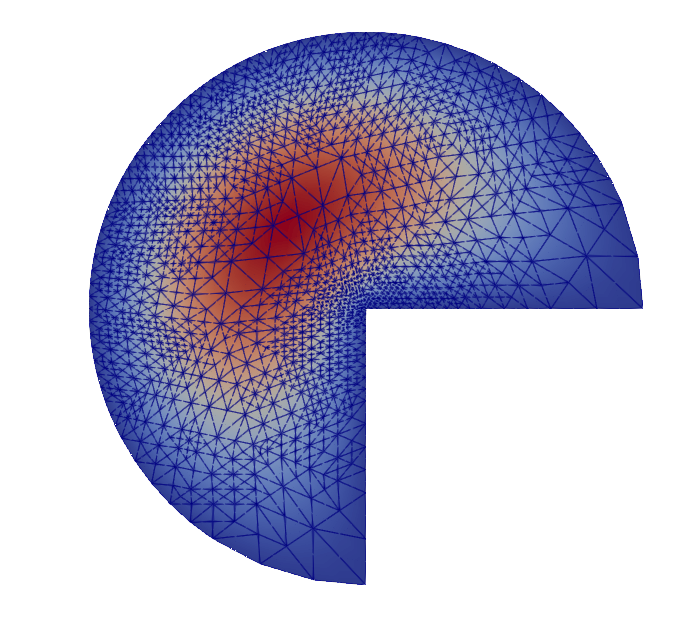
\includegraphics[scale=0.2]{Figures/Pacman.png}
			\end{figure}
			\vspace{0.3cm}
		\end{minipage}
	\end{frame}
	\begin{frame}
		\frametitle{ngsPETSc -- Firedrake}
		$\newline$
		\textbf{ngsPETSc} provides new capabilities to \textbf{Firedrake} such as:
		$\newline$
		\begin{itemize}
			\item[\color{oxfordblue}$\blacktriangleright$] Access to all Netgen generated linear meshes and high order meshes.
			\item[\color{oxfordblue}$\blacktriangleright$] Splits for macro elements, such as Alfeld splits and Powell-Sabin splits (even on curved geometries).
			\item[\color{oxfordblue}$\blacktriangleright$] Adaptive mesh refinement capabilities, that conform to the geometry.
			\item[\color{oxfordblue}$\blacktriangleright$] High order meshes hierarchy for multigrid solvers.
		\end{itemize}
	\end{frame}
	\begin{frame}{Examples -- Opencascade via NETGEN}
		\lstinputlisting[language=python,firstline=4,lastline=14]{Examples/occ.py}
	\end{frame}
	\begin{frame}{Examples -- Opencascade via NETGEN}
		$\newline$
		\lstinputlisting[language=python,firstline=15,lastline=17]{Examples/occ.py}
	\begin{figure}
			\centering
			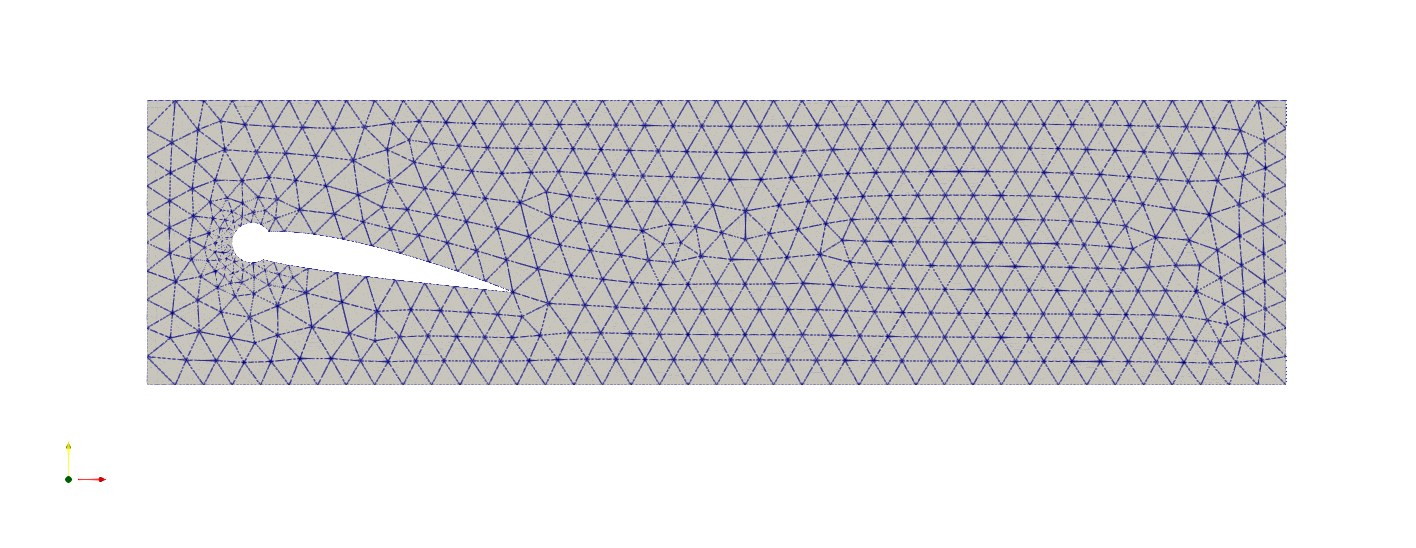
\includegraphics[scale=0.2]{Figures/nacaMesh.png}
		\end{figure}	
	\end{frame}
	\begin{frame}{Stokes flow -- Weak formulation}
		$\newline$
		Find $(\vec{u},p) \in V \times Q$ such that
		\begin{align*}
			\int_{\Omega} \nabla \vec{u} : \nabla \vec{v} - \int_{\Omega} p \nabla \cdot \vec{v} &= \int_{\Omega} \vec{f} \cdot \vec{v} \quad &\forall \vec{v} \in V \\
			\int_{\Omega} q \nabla \cdot \vec{u} &= 0 \quad &\forall q \in Q
		\end{align*}
		where $V$ and $Q$ are the velocity and pressure spaces respectively, i.e. $V = H^1_0(\Omega)^2$ and $Q = L^2_0(\Omega)$.
	\end{frame}
	\begin{frame}
		\frametitle{Stokes flow -- Inf-sup condition}
		$\newline$
		$\newline$
		We can also look for a discrete solution, i.e. find $(\vec{u}_h,p_h) \in V_h \times Q_h$ such that	
		\begin{minipage}{0.75\textwidth}
			\begin{gather}
				\nu\int_{\Omega} \nabla \vec{u} : \nabla \vec{v} - \int_{\Omega} p \nabla \cdot \vec{v} = \int_{\Omega} \vec{f} \cdot \vec{v}\\
				\int_{\Omega} q \nabla \cdot \vec{u} = 0
			\end{gather}
		for all $(\vec{v},q) \in V_h \times Q_h$.
		\begin{equation}
			\underset{q\in Q_h}{\inf} \underset{\vec{v}\in V_h}{\sup} \frac{\int_{\Omega} q \nabla \cdot \vec{v}}{\norm{q}_{L^2} \norm{\vec{v}}_{H^1}} \geq \beta > 0	
		\end{equation}
		\end{minipage}
		\begin{minipage}{0.2\textwidth}
			\begin{figure}
				\centering
				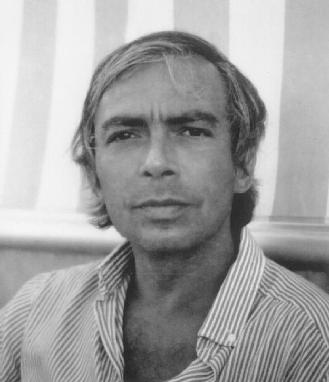
\includegraphics[scale=0.2]{Figures/Brezzi.jpg}
				\begin{center}
					\small Franco Brezzi
				\end{center}
			\end{figure}
		\end{minipage}
	\end{frame}
	\begin{frame}
		\frametitle{Stokes flow -- UFL}
		$\newline$
		\lstinputlisting[language=python,firstline=27,lastline=31]{Examples/scottVogelius.py}
	\end{frame}
	\begin{frame}
		\frametitle{Stokes flow -- Scott--Vogelius element}
		$\newline$
		$\newline$
		We can use the Scott--Vogelius pair, which is a mixed finite element of order $k$ for the velocity and order $k-1$ for the pressure.
		Such an element is inf-sup stable for $k \geq 2$, under certain assumptions on the mesh. Such pair is \textbf{divergence-free}.
		\begin{minipage}{0.75\textwidth}
			$\newline$	
			When $k=2$ we need \textbf{Alfeld splits}.
			\lstinputlisting[language=python,firstline=17,lastline=19]{Examples/scottVogelius.py}
			\lstinputlisting[language=python,firstline=24,lastline=26]{Examples/scottVogelius.py}
		\end{minipage}
		\begin{minipage}{0.2\textwidth}
			\begin{figure}
				\centering
				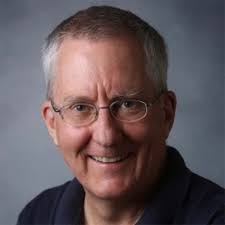
\includegraphics[scale=0.3]{Figures/Scott.jpeg}
				\begin{center}
					\small Ridgway Scott
				\end{center}
			\end{figure}
		\end{minipage}
	\end{frame}
	\begin{frame}
		\frametitle{Stokes flow -- Scott--Vogelius}
		$\newline$
		\lstinputlisting[language=python,firstline=38,lastline=41]{Examples/scottVogelius.py}
		\vspace{-1cm}
		\begin{figure}
			\centering
			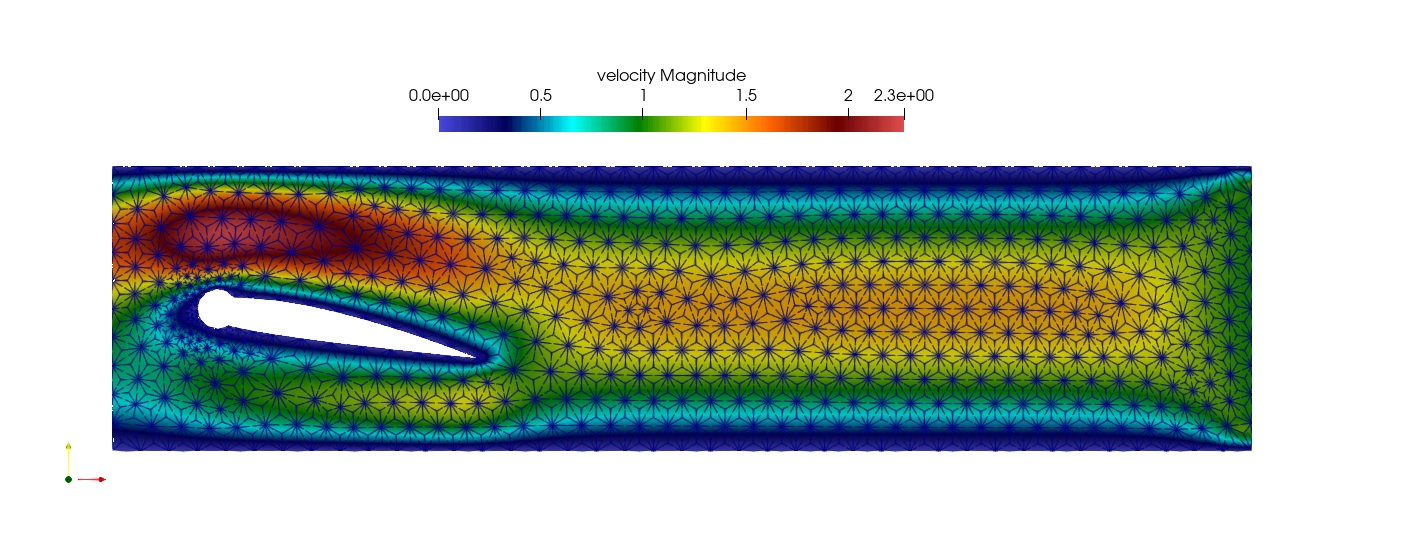
\includegraphics[scale=0.2]{Figures/scottVogelius.png}
		\end{figure}
	\end{frame}
	\begin{frame}
		\frametitle{Stokes flow -- Hood--Taylor element}
		$\newline$
		$\newline$
		Another element pair we will use is the Hood--Taylor pair, which has \textbf{no restrictions} on the mesh in two dimensions.
		$\newline$
		$\newline$
		\begin{minipage}{0.8\textwidth}
			\lstinputlisting[language=python,firstline=24,lastline=26]{Examples/hoodTaylor.py}
			\textbf{We lose the point-wise divergence-free property!}
			This is not an issue because the same would happen for Scott-Vogelius on curved meshes.
		\end{minipage}
		\begin{minipage}{0.18\textwidth}
			\begin{figure}
				\centering
				\qquad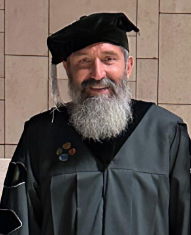
\includegraphics[scale=0.4]{Figures/Boffi.png}
				\begin{center}
					\small Daniele Boffi
				\end{center}
			\end{figure}
		\end{minipage}
	\end{frame}
	\begin{frame}{Fieldsplit Schur preconditioner}
		$\newline$
		$\newline$
		The previous set of equations can be written in matrix form as
		\vspace{-0.3cm}
		\begin{equation}
			\begin{bmatrix}
				A & B^T \\
				B & 0
			\end{bmatrix}
			\begin{bmatrix}\vec{u} \\p\end{bmatrix}=\begin{bmatrix}\vec{f} \\0\end{bmatrix}
		\end{equation}
		We choose as preconditioner the \textbf{fieldsplit Schur preconditioner}, i.e.
		\vspace{-0.3cm}
		\begin{equation}
			\begin{bmatrix}
				I & -\hat{A}^{-1} B^T\\
				0 & I
			\end{bmatrix}
			\begin{bmatrix}
				\hat{A}^{-1}& 0\\
				0 & \hat{S}^{-1}
			\end{bmatrix}
			\begin{bmatrix}
				I & 0\\
				-B\hat{A}^{-1} & I
			\end{bmatrix}
		\end{equation}
		where $S$ is the \textbf{Schur complement}, i.e. $S = -BA^{-1}B^T$.
		\lstinputlisting[language=python, firstline=18, lastline=21]{Examples/solvers.py}
	\end{frame}
	\begin{frame}
		\frametitle{Fieldsplit Schur preconditioner -- Mass matrix}
		$\newline$
		$\newline$
		Thanks to the inf-sup condition we can prove that the Schur complement is spectrally equivalent to the mass matrix, hence we can use as preconditioner:
		\begin{minipage}{0.7\textwidth}
			\vspace{-0.35cm}
			\begin{equation}
				\begin{bmatrix}
					I & -\hat{A}^{-1} B^T\\
					0 & I
				\end{bmatrix}
				\begin{bmatrix}
					\hat{A}^{-1}& 0\\
					0 & -\nu \hat{M}^{-1}
				\end{bmatrix}
				\begin{bmatrix}
					I & 0\\
					-B\hat{A}^{-1} & I
				\end{bmatrix}
			\end{equation}
			where $M$ is the mass matrix.
			\lstinputlisting[language=python,firstline=43,lastline=47]{Examples/multigrid.py}
		\end{minipage}
		\begin{minipage}{0.28\textwidth}
			\begin{figure}
				\centering
				\qquad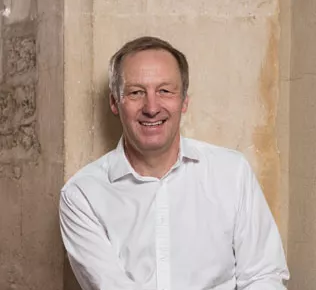
\includegraphics[scale=0.35]{Figures/Wathen.png}
				\begin{center}
					\small Andrew Wathen
				\end{center}
			\end{figure}
		\end{minipage}
	\end{frame}
	\begin{frame}{Multigrid on curved meshes}
		$\newline$
		ngsPETSc allows us to create a hierarchy of curved meshes for multigrid solvers.
		\lstinputlisting[language=python,firstline=19,lastline=21]{Examples/multigrid.py}
		We can than use a multigrid solver to compute $\hat{A}^{-1}$:
		\lstinputlisting[language=python,firstline=18,lastline=23]{Examples/solvers.py}
	\end{frame}
	\begin{frame}{Monolithic multigrid on curved meshes -- Coarse mesh}
		$\newline$
		We can also a monolithic multigrid solver for the Schur complement:
		\lstinputlisting[language=python,firstline=30,lastline=38]{Examples/solvers.py}
	\end{frame}
	\begin{frame}{Monolithic multigrid on curved meshes -- Fine mesh}
		$\newline$
		\lstinputlisting[language=python,firstline=43,lastline=53]{Examples/solvers.py}
	\end{frame}
	\begin{frame}{Navier-Stokes flow}
		A more interesting example is the Navier-Stokes flow, which is a non-linear problem.
		In particular, we will consider the problem of finding $(\vec{u},p) \in H^1(\Omega)^2\times L^2_0(\Omega)$ such that
		\begin{align*}
			\int_\Omega \partial_t \vec{u} \cdot \vec{v} + \int_\Omega(\nabla \vec{u})\vec{u}\cdot\vec{v}+\nu\int_{\Omega} \nabla \vec{u} : \nabla \vec{v} - \int_{\Omega} p \nabla \cdot \vec{v} &= \int_{\Omega} \vec{f} \cdot \vec{v}\\
			\int_{\Omega} q \nabla \cdot \vec{u} &= 0
		\end{align*}
		for all $(\vec{v},q) \in H^1(\Omega)^2\times L^2_0(\Omega)$.
	\end{frame}
	\begin{frame}{Navier-Stokes flow -- Augmented Lagrangian}
		$\newline$
		We consider an augmented Lagrangian formulation for the discrete problem, i.e. find $(\vec{u}_h,p_h) \in V_h \times Q_h$ such that
		\begin{align*}
			(\partial_t\vec{u},\vec{v})_0 + (\nabla \vec{u}\vec{u},\vec{v})_0 &+ \nu(\nabla \vec{u},\nabla \vec{v})_0 \\
			 & - (p,\nabla \cdot \vec{v})_0 + \frac{\gamma}{2}(\nabla \cdot \vec{u},\nabla \cdot \vec{v})_0 &= (\vec{f},\vec{v})_0\\
		\end{align*}
		and verifying the weak divergence free constraint $(\nabla \cdot \vec{u},q)_0 = 0$, for all $(\vec{v},q) \in V_h \times Q_h$.
	\end{frame}
	\begin{frame}
		\frametitle{Navier-Stokes flow -- Fieldsplit Schour preconditioner}
		$\newline$
		$\newline$
		The linearized version of the Navier-Stokes equations can be written in matrix form as 
		\vspace{-0.3cm}
		\begin{equation}
			\begin{bmatrix}
				A+\gamma B^TWB& B^T \\
				B & 0
			\end{bmatrix}
			\begin{bmatrix}\vec{u} \\p\end{bmatrix}=\begin{bmatrix}\vec{f} \\0\end{bmatrix}
		\end{equation}
		We choose as preconditioner the \textbf{fieldsplit Schur preconditioner}, i.e.
		\vspace{-0.3cm}
		\begin{equation}
			\begin{bmatrix}
				I & -\hat{A}_\gamma^{-1} B^T\\
				0 & I
			\end{bmatrix}
			\begin{bmatrix}
				\hat{A}_\gamma^{-1}& 0\\
				0 & \hat{S}_\gamma^{-1}
			\end{bmatrix}
			\begin{bmatrix}
				I & 0\\
				-BA_\gamma^{-1} & I
			\end{bmatrix}
		\end{equation}
		\begin{equation}
			A_\gamma = A+\gamma B^TWB 	\qquad  S_\gamma = -BA_\gamma^{-1}B^T.
		\end{equation}
		In this case, we notice that independently of the Reynolds numbers $S_\gamma\sim - (\nu+\gamma)^{-1} M$.
	\end{frame}
	\begin{frame}{Navier-Stokes flow -- Augmented Lagrangian}
		$\newline$
		\begin{itemize}
			\item [\color{oxfordblue}$\blacktriangleright$] The augmented Lagrangian term helps enforce the divergence-free constraint, and makes the scheme pressure robuts.
			\item [\color{oxfordblue}$\blacktriangleright$] We can use as preconditioner
			\begin{equation}
				\begin{bmatrix}
					I & -\hat{A}_\gamma^{-1} B^T\\
					0 & I
				\end{bmatrix}
				\begin{bmatrix}
					\hat{A}_\gamma^{-1}& 0\\
					0 & -(\nu+\gamma)M^{-1}
				\end{bmatrix}
				\begin{bmatrix}
					I & 0\\
					-BA_\gamma^{-1} & I
				\end{bmatrix}
			\end{equation}
			\item[\color{oxfordblue}$\blacktriangleright$] How do we compute $\hat{A}_\gamma^{-1}$ efficiently ? Can we adopt a multigrid approach ?
		\end{itemize}
	\end{frame}
	\begin{frame}
		\frametitle{Subspace correction methods for nearly singular
problems}
		$\newline$
		$\newline$
		To compute $\hat{A}_\gamma^{-1}$ we can use a subspace correction method.
		We decompose the space $V_h$ as follows:
		\vspace{-0.3cm}
		\begin{equation}
			V_h = \sum_{i=1} V_i.
		\end{equation}
		We consider a coarse space $V_H$ and the projection and injection operators:
		\vspace{-0.3cm}
		\begin{equation}
			P_H : V_H \rightarrow V_h, \qquad I : V_h \rightarrow V_i.
		\end{equation}
		We then consider as smoother the additive Schwarz preconditioner defined as:
		\begin{equation}
			\hat{A}_\gamma^{-1} = P_H A_{\gamma,H}^{-1} P_H^T + \sum_{i=1} I_i A_{\gamma,i}^{-1} I_i^T.
		\end{equation}
	\end{frame}
	\begin{frame}
		\frametitle{Subspace correction methods for nearly singular
problems}
		$\newline$
		\begin{block}{Robust relaxetion}
			We need the discrete kernel,
			\vspace{-0.3cm}
			\begin{equation}
				\mathbb{K}_h =  \{\vec{v} \in V_h : B\vec{v} = 0\},
			\end{equation}
			to decompose in a \textbf{stable} way as follows:
			\vspace{-0.3cm}
			\begin{equation}
				\mathbb{K}_h = \sum_{i=1} \mathbb{K}_h\cap V_i.
			\end{equation}
		\end{block}
	\end{frame}
	\begin{frame}[fragile]
		\frametitle{Robust relaxation -- Hood--Taylor}
		\begin{equation*}
			\begin{tikzcd}[row sep=huge]
			0 \arrow[r,""] & \Big[H^2(\Omega)\Big]^2 \arrow[r,"\curl"] \arrow[d]& \Big[H^1_0(\Omega)\Big]^2 \arrow[r,"\div"] \arrow[d]& L^2_0(\Omega) \arrow[r,""]\arrow[d] & 0\\
			0 \arrow[r,""] & \Big[\mathbb{P}^4(\mathcal{T}_h)\Big]^2 \arrow[r,"\curl"] & \Big[\mathbb{P}^3(\mathcal{T}_h)\Big]^2 \arrow[r,"\div"] & \mathbb{P}^2_{disc}(\mathcal{T}_h) \arrow[r,""] & 0\\
			\end{tikzcd}
		\end{equation*}
		\vspace{-2cm}
		\begin{figure}[h]
			\centering
			\hspace{1cm}\scalebox{0.45}{\tikzfig{Figures/DoF}}
		\end{figure}
	\end{frame}
	\begin{frame}
		\frametitle{Robust prolongation -- Hood--Taylor}
		$\newline$
		\begin{block}{Robust relaxetion}
			If the space pair $(V_h,Q_h)$ is inf-sup stable and the mesh we have a robust prolongation operator defined by:
			\begin{equation}
				\tilde P_H \vec{u}_H - \tilde{\vec{u}}_h = \vec{u}_H-\tilde{\vec{u}}_h,
			\end{equation}
			where
			\begin{equation}
				a_{\gamma}(\tilde{\vec{u}}_h,\tilde{\vec{v}}_h) = \gamma(\nabla \cdot \tilde{\vec{u}}_h,\nabla \cdot \tilde{\vec{v}}_h)_{\pi_{Q_h}\pi{Q_h}^T} \quad \forall \tilde{\vec{v}}_h \in \tilde{V}_h,
			\end{equation}
			where $\pi_{Q_h}$ is the $L^2$ projection onto $Q_h$ and $\tilde{V}_h$ is the space of discrete velocity vanishing at the boundary of the coarse cells.
		\end{block}
	\end{frame}
	\begin{frame}
		\frametitle{Numerical Simulation}
		\begin{figure}
			\centering
			\scalebox{0.2}{\animategraphics[loop,autoplay]{12}{Figures/NS/Velocity.}{0000}{0158}}
		\end{figure}
	\end{frame}
\end{document}


\pgfdeclareimage[width=\paperwidth]{titlebackground}{Images/title-slide-background.png}
\setbeamerfont{subtitle}{size=\tiny}
\setbeamertemplate{endpage}{
	\begin{picture}(0,0)
		\scalebox{1.01}{
		\put(-28.5,-163){%
			\pgfuseimage{titlebackground}
		}
		}
		\put(0,-115){%
			\begin{minipage}[b][4.5cm][t]{0.5\textwidth}
				\color{white}
				\usebeamerfont{title}
				{\textbf{Thank Your} \\ \textbf{For You Attention !}}
			\end{minipage}
		}
	\end{picture}
}
\setbeamertemplate{title page}{
	\begin{picture}(0,0)
		\scalebox{1.01}{
			\put(-28.5,-163){%
				\pgfuseimage{titlebackground}
			}
		}
		\put(0,-60){%
			\begin{minipage}[b][4.5cm][t]{0.7\textwidth}
				\color{white}
				\usebeamerfont{title}
				{\inserttitle\\[0.9cm]}
				\usebeamerfont{subtitle}
				{\insertauthor\par}
				{\insertinstitute\\[0.3cm]}
				{\insertdate}
			\end{minipage}
		}
	\end{picture}
}


%% General slide formatting %%

\definecolor{oxfordblue}{RGB}{4,30,66}
\definecolor{oxfordred}{RGB}{207,48,42}

\pgfdeclareimage[width=0.9cm]{oxfordlogo}{Images/oxford-logo.png}
\pgfdeclareimage[width=1cm]{mathslogo}{Images/mathematics-logo.png}
\pgfdeclareimage[width=1.2cm]{ngslogo}{Images/ngs-logo.png}
\pgfdeclareimage[width=1.2cm]{petsclogo}{Images/petsc-logo.png}
\pgfdeclareimage[width=1.2cm]{firedrakelogo}{Images/firedrake-logo.png}

\setbeamertemplate{headline}
{%
	\begin{picture}(0,0)
		\put(314,-50){%
			\pgfuseimage{oxfordlogo}
		}
		\put(20,-55){%
			\rule{320pt}{0.4pt}
		}
	\end{picture}
}
\def\ngshead{
	\begin{picture}(0,0)
		\put(278,0){%
			\pgfuseimage{ngslogo}
		}
		\put(-8,-5){%
			\rule{325pt}{0.4pt}
		}
	\end{picture}
}
\def\petschead{
	\begin{picture}(0,0)
		\put(278,0){%
			\pgfuseimage{petsclogo}
		}
		\put(-8,-5){%
			\rule{325pt}{0.4pt}
		}
	\end{picture}
}
\def\firedrakehead{
	\begin{picture}(0,0)
		\put(278,0){%
			\pgfuseimage{firedrakelogo}
		}
		\put(-8,-5){%
			\rule{325pt}{0.4pt}
		}
	\end{picture}
}
\setbeamertemplate{frametitle}
{%
	\begin{picture}(0,0)
		\put(-8,-20){%
			\normalsize\textbf{\color{oxfordblue}\insertframetitle}
		}
		\put(-8,-32){%
			\normalsize\textbf{\color{oxfordblue}\insertframesubtitle}
		}
	\end{picture}
}

\setbeamertemplate{footline}
{%
	\begin{picture}(0,0)
		\put(20,30){%
			\rule{320pt}{0.4pt}
		}
		\put(20,14){%
			\pgfuseimage{mathslogo}
		}
		\put(100,14){%
			\color{oxfordblue}\insertshortdate
		}
		\put(160,14){%
			\color{oxfordblue}\insertshorttitle
		}
		\put(337,14){%
			\color{oxfordblue}\insertframenumber
		}
	\end{picture}%
}
\def\footer{
	\begin{picture}(0,0)
		\put(-308,-75){%
			\rule{325pt}{0.4pt}
		}
		\put(-308,-91){%
			\pgfuseimage{mathslogo}
		}
		\put(-228,-91){%
			\color{oxfordblue}\tiny\insertshortdate
		}
		\put(-168,-91){%
			\color{oxfordblue}\tiny\insertshorttitle
		}
		\put(9,-91){%
			\color{oxfordblue}\tiny\insertframenumber
		}
	\end{picture}
}

\setbeamercolor{block title}{bg=oxfordblue!30,fg=black}
\setbeamercolor{palette primary}{bg=oxfordblue,fg=white}

\definecolor{codegreen}{rgb}{0,0.6,0}
\definecolor{codegray}{rgb}{0.5,0.5,0.5}
\definecolor{codepurple}{rgb}{0.58,0,0.82}
\definecolor{backcolour}{rgb}{0.95,0.95,0.92}

\lstdefinestyle{mystyle}{
	%backgroundcolor=\color{backcolour},   
	commentstyle=\color{codegray},
	keywordstyle=\color{oxfordblue},
	numberstyle=\tiny\color{codegray},
	stringstyle=\color{codegreen},
	basicstyle=\ttfamily\footnotesize,
	breakatwhitespace=false,         
	breaklines=true,                 
	captionpos=b,                    
	keepspaces=true,                 
	numbers=left,                    
	numbersep=5pt,                  
	showspaces=false,                
	showstringspaces=false,
	showtabs=false,                  
	tabsize=2
}
\AtBeginSection[]{
  \begin{frame}
  \vfill
  \centering
  \begin{beamercolorbox}[sep=8pt,center,shadow=true,rounded=true]{title}
    \usebeamerfont{title}\insertsectionhead\par%
  \end{beamercolorbox}
  \vfill
  \end{frame}
}

\lstset{style=mystyle}

%% Information (author, title, etc.) %%
\title[ngsPETSc]{ngsPETSc: NETGEN meets PETSc} % short title for footer
\author%
{%
	\sc{P.~E.~Farrell}*, \sc{S.~Zampini$\dag$}, \underline{\sc{U.~Zerbinati}}*\\
}
\institute%
{%
	* \textit{Mathematical Institute}\\
	\;\textit{University of Oxford}\\
	$\newline$
	$\dag$ \textit{Extreme Computing Research Center}\\
	\;\textit{King Abdullah University of Science and Technology}\\	
}

\date[\textbf{DD28}]{28 International Conference on Domain Decomposition Methods, 29th Jannuary 2024, KAUST} % short date for footer



%% Content of slides %%

\begin{document}
	\begin{frame}[plain]
		\titlepage
	\end{frame}
	\begin{frame}[plain]
		\frametitle{NETGEN}
		\ngshead
		$\newline$
		$\newline$
		NETGEN is an advancing front 2D/3D-mesh generator, with many interesting features.
		$\newline$
		$\newline$
		\begin{minipage}{0.58\textwidth}
			\begin{itemize}
				\item[\color{oxfordblue}$\blacktriangleright$] The geometry we intend to mesh can be described by \textbf{Constructive Solid Geometry} (CSG), in particular we can use \textbf{Opencascade} to describe our geometry.
				\item[\color{oxfordblue}$\blacktriangleright$] It is able to construct isoparametric meshes, which conform to the geometry.
			\end{itemize}
		\end{minipage}
		\qquad
		\begin{minipage}{0.3\textwidth}
			\begin{figure}
				\centering
				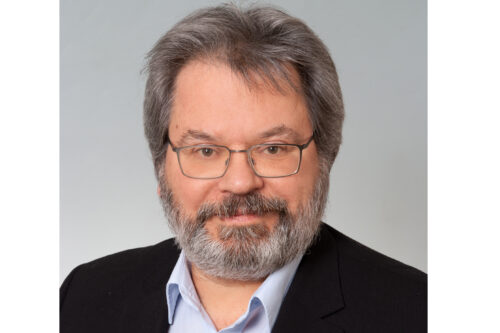
\includegraphics[scale=1.]{Figures/Schoeberl.jpg}
				\begin{center}
					\qquad\small Joachim Sc\"{o}berl
				\end{center}
			\end{figure}
			\vspace{0.3cm}
		\end{minipage}
	\end{frame}

	\begin{frame}[plain]
		$\newline$ 
		$\newline$ 
		\frametitle{PETSc}
		\petschead
		$\newline$
		$\newline$ 
		PETSc stands for Portable, Extensible Toolkit for Scientific Computation, is a library for the scalable (parallel) solution of scientific applications modeled by partial differential equations (PDEs).
		$\newline$
		\begin{minipage}{0.58\textwidth}
			\begin{itemize}
				\item[\color{oxfordblue}$\blacktriangleright$] \textbf{PETSc KSP} provides access to extremly efficent Krylov solvers.
				\item[\color{oxfordblue}$\blacktriangleright$] \textbf{PETSc SNES} provides access to extremly efficent non-linear solvers, with line-searching and trust region capabilities.
			\end{itemize}
		\end{minipage}
		\qquad
		\begin{minipage}{0.3\textwidth}
			\begin{figure}
				\centering
				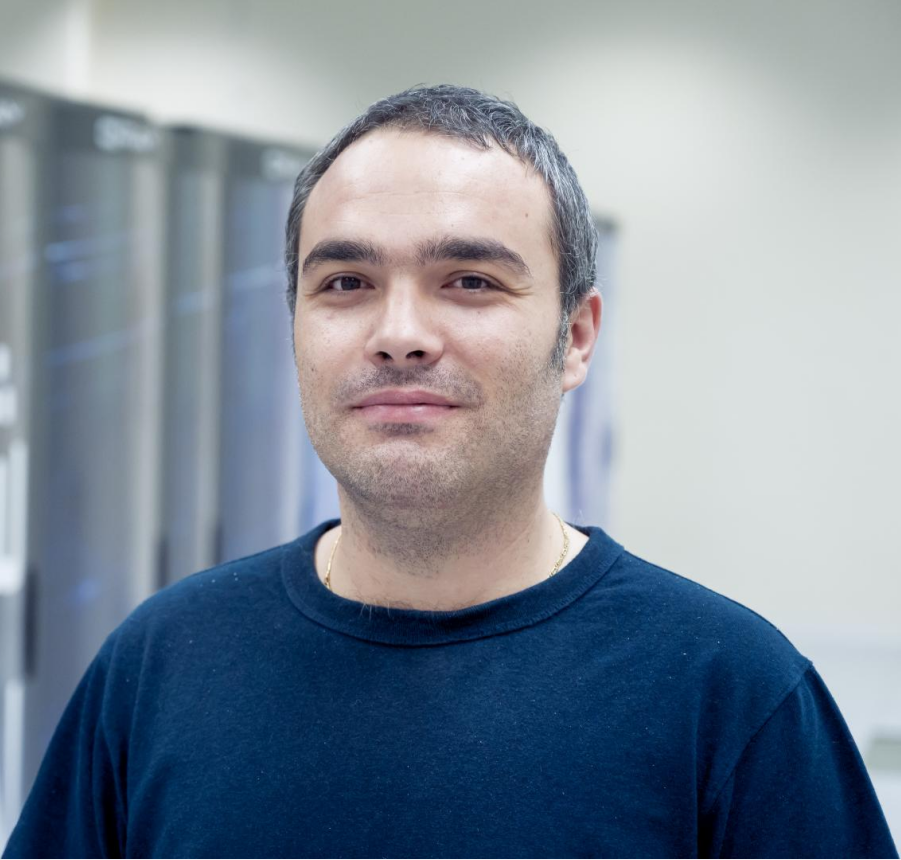
\includegraphics[scale=0.15]{Figures/Zampini.png}
				\begin{center}
					\;\;\small Stefano Zampini
				\end{center}
			\end{figure}
		\end{minipage}
		\vspace{3cm}
	\end{frame}
	\begin{frame}
		\frametitle{ngsPETSc -- NETGEN/NGSolve}
		$\newline$
		\textbf{ngsPETSc} is an interface between NETGEN/NGSolve and \textbf{PETSc}. In particular, \textbf{ngsPETSc} provides new capabilities to \textbf{NETGEN}/\textbf{NGSolve} such as:
		$\newline$
		\begin{itemize}
			\item[\color{oxfordblue}$\blacktriangleright$] Access to all linear solver capabilities of \textbf{KSP}.
			\item[\color{oxfordblue}$\blacktriangleright$] Access to all preconditioning capabilities of \textbf{PC}.
			\item[\color{oxfordblue}$\blacktriangleright$] Access to all non-linear solver capabilities of \textbf{SNES}.
			\item[\color{oxfordblue}$\blacktriangleright$] Access to all mesh refinement capabilities of \textbf{DMPLEX}.
		\end{itemize}
	\end{frame}
	\begin{frame}[plain]
		$\newline$ 
		\petschead
		\frametitle{PETSc DMPlex}
		$\newline$ 
		$\newline$
		\begin{minipage}{0.58\textwidth}
			\textbf{PETSc DMPlex} handles unstructured grids using the generic \textbf{PETSc} interface for hierarchy and multi-physics. 
			$\newline$
			\begin{itemize}
				\item[\color{oxfordblue}$\blacktriangleright$] \textbf{PETSc DMPlex} provides a wide variety of primitive mesh operations such as: \textit{meet}, \textit{clousre}, \textit{cone}, etc
				\item[\color{oxfordblue}$\blacktriangleright$] \textbf{PETSc DMPlex} provides a wide variety of mesh refinement operations such as: \textit{unifrom refinement}, \textit{Alfeld refinement}, \textit{box refinement}, etc
			\end{itemize}
		\end{minipage}
		\qquad
		\begin{minipage}{0.33\textwidth}
			\begin{figure}
				\centering
				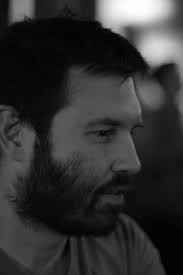
\includegraphics[scale=0.5]{Figures/Kneply.jpeg}
				\begin{center}
					\hspace{0.5cm}\small Matthew G.~Knepley
				\end{center}
			\end{figure}
		\end{minipage}
	\end{frame}
	\begin{frame}[plain]
		\firedrakehead
		$\newline$
		$\newline$
		\textbf{Firedrake} is an automated system for the solution of partial differential equations using the finite element method (FEM).
		$\newline$
		$\newline$
		\begin{minipage}{0.58\textwidth}
			\begin{itemize}
				\item[\color{oxfordblue}$\blacktriangleright$] Variational formulation can be easily defined using the \textbf{UFL} language.
				\item[\color{oxfordblue}$\blacktriangleright$] Wide class of finite elements are available, including $H(div)$, $H(curl)$, $H^1$ and $H^2$.
				\item[\color{oxfordblue}$\blacktriangleright$] Provides access to \textbf{PETSc} linear solvers and non-linear solvers.
			\end{itemize}
		\end{minipage}
		\qquad
		\begin{minipage}{0.3\textwidth}
			\begin{figure}
				\centering
				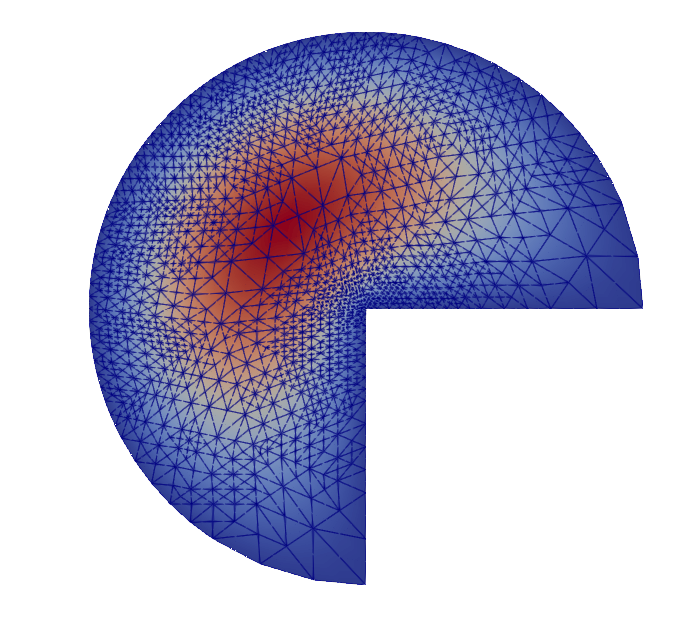
\includegraphics[scale=0.2]{Figures/Pacman.png}
			\end{figure}
			\vspace{0.3cm}
		\end{minipage}
	\end{frame}
	\begin{frame}
		\frametitle{ngsPETSc -- Firedrake}
		$\newline$
		\textbf{ngsPETSc} provides new capabilities to \textbf{Firedrake} such as:
		$\newline$
		\begin{itemize}
			\item[\color{oxfordblue}$\blacktriangleright$] Access to all Netgen generated linear meshes and high order meshes.
			\item[\color{oxfordblue}$\blacktriangleright$] Splits for macro elements, such as Alfeld splits and Powell-Sabin splits (even on curved geometries).
			\item[\color{oxfordblue}$\blacktriangleright$] Adaptive mesh refinement capabilities, that conform to the geometry.
			\item[\color{oxfordblue}$\blacktriangleright$] High order meshes hierarchy for multigrid solvers.
		\end{itemize}
	\end{frame}
	\begin{frame}{Examples -- Opencascade via NETGEN}
		\lstinputlisting[language=python,firstline=4,lastline=14]{Examples/occ.py}
	\end{frame}
	\begin{frame}{Examples -- Opencascade via NETGEN}
		$\newline$
		\lstinputlisting[language=python,firstline=15,lastline=17]{Examples/occ.py}
	\begin{figure}
			\centering
			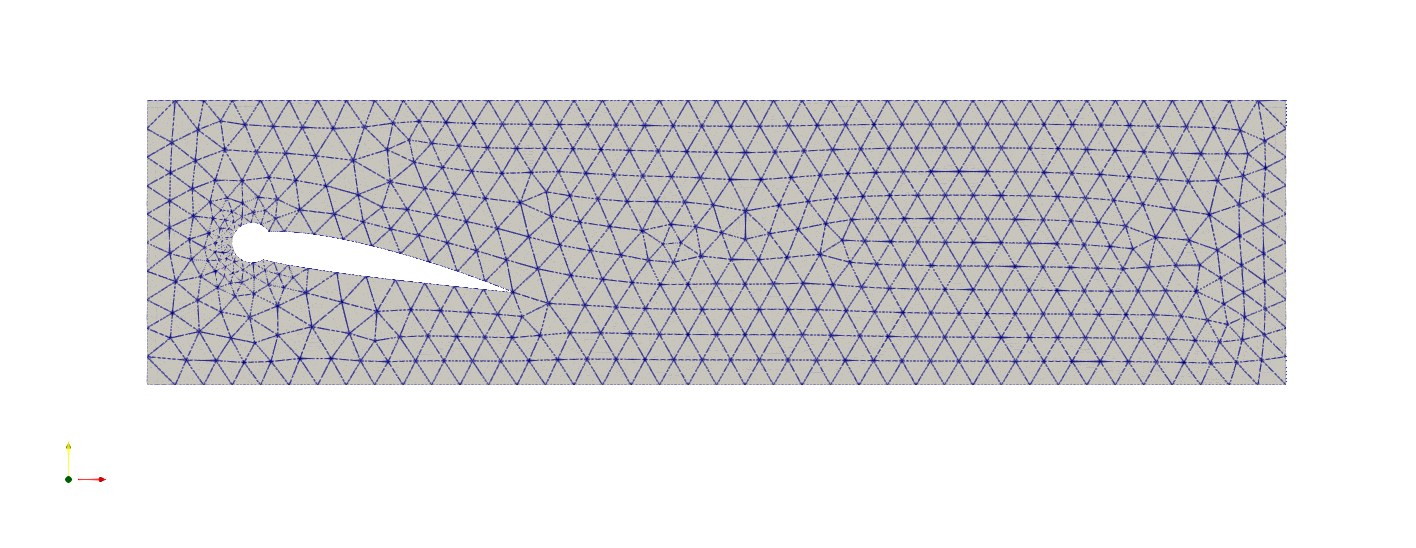
\includegraphics[scale=0.2]{Figures/nacaMesh.png}
		\end{figure}	
	\end{frame}
	\begin{frame}{Stokes flow -- Weak formulation}
		$\newline$
		Find $(\vec{u},p) \in V \times Q$ such that
		\begin{align*}
			\int_{\Omega} \nabla \vec{u} : \nabla \vec{v} - \int_{\Omega} p \nabla \cdot \vec{v} &= \int_{\Omega} \vec{f} \cdot \vec{v} \quad &\forall \vec{v} \in V \\
			\int_{\Omega} q \nabla \cdot \vec{u} &= 0 \quad &\forall q \in Q
		\end{align*}
		where $V$ and $Q$ are the velocity and pressure spaces respectively, i.e. $V = H^1_0(\Omega)^2$ and $Q = L^2_0(\Omega)$.
	\end{frame}
	\begin{frame}
		\frametitle{Stokes flow -- Inf-sup condition}
		$\newline$
		$\newline$
		We can also look for a discrete solution, i.e. find $(\vec{u}_h,p_h) \in V_h \times Q_h$ such that	
		\begin{minipage}{0.75\textwidth}
			\begin{gather}
				\nu\int_{\Omega} \nabla \vec{u} : \nabla \vec{v} - \int_{\Omega} p \nabla \cdot \vec{v} = \int_{\Omega} \vec{f} \cdot \vec{v}\\
				\int_{\Omega} q \nabla \cdot \vec{u} = 0
			\end{gather}
		for all $(\vec{v},q) \in V_h \times Q_h$.
		\begin{equation}
			\underset{q\in Q_h}{\inf} \underset{\vec{v}\in V_h}{\sup} \frac{\int_{\Omega} q \nabla \cdot \vec{v}}{\norm{q}_{L^2} \norm{\vec{v}}_{H^1}} \geq \beta > 0	
		\end{equation}
		\end{minipage}
		\begin{minipage}{0.2\textwidth}
			\begin{figure}
				\centering
				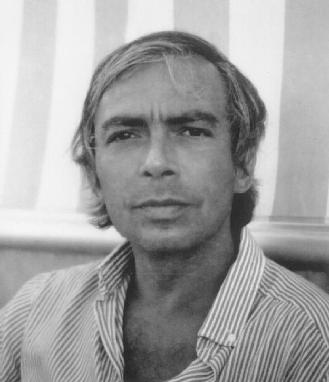
\includegraphics[scale=0.2]{Figures/Brezzi.jpg}
				\begin{center}
					\small Franco Brezzi
				\end{center}
			\end{figure}
		\end{minipage}
	\end{frame}
	\begin{frame}
		\frametitle{Stokes flow -- UFL}
		$\newline$
		\lstinputlisting[language=python,firstline=27,lastline=31]{Examples/scottVogelius.py}
	\end{frame}
	\begin{frame}
		\frametitle{Stokes flow -- Scott--Vogelius element}
		$\newline$
		$\newline$
		We can use the Scott--Vogelius pair, which is a mixed finite element of order $k$ for the velocity and order $k-1$ for the pressure.
		Such an element is inf-sup stable for $k \geq 2$, under certain assumptions on the mesh. Such pair is \textbf{divergence-free}.
		\begin{minipage}{0.75\textwidth}
			$\newline$	
			When $k=2$ we need \textbf{Alfeld splits}.
			\lstinputlisting[language=python,firstline=17,lastline=19]{Examples/scottVogelius.py}
			\lstinputlisting[language=python,firstline=24,lastline=26]{Examples/scottVogelius.py}
		\end{minipage}
		\begin{minipage}{0.2\textwidth}
			\begin{figure}
				\centering
				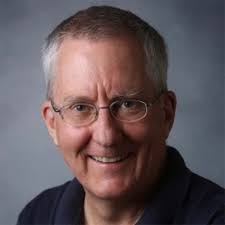
\includegraphics[scale=0.3]{Figures/Scott.jpeg}
				\begin{center}
					\small Ridgway Scott
				\end{center}
			\end{figure}
		\end{minipage}
	\end{frame}
	\begin{frame}
		\frametitle{Stokes flow -- Scott--Vogelius}
		$\newline$
		\lstinputlisting[language=python,firstline=38,lastline=41]{Examples/scottVogelius.py}
		\vspace{-1cm}
		\begin{figure}
			\centering
			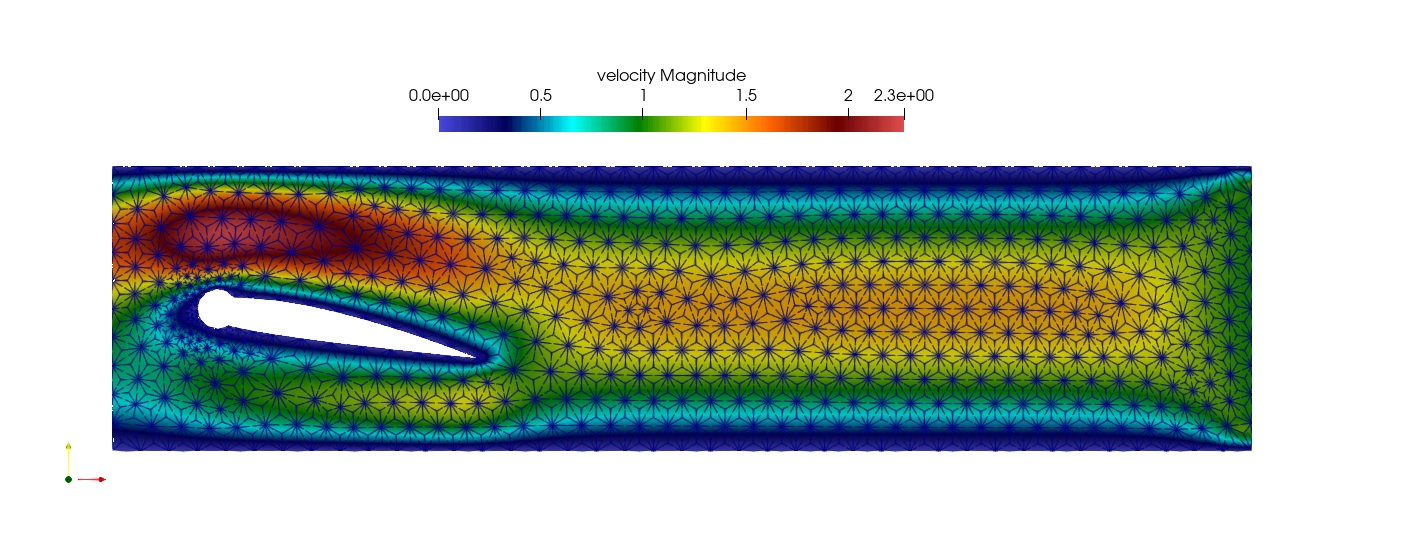
\includegraphics[scale=0.2]{Figures/scottVogelius.png}
		\end{figure}
	\end{frame}
	\begin{frame}
		\frametitle{Stokes flow -- Hood--Taylor element}
		$\newline$
		$\newline$
		Another element pair we will use is the Hood--Taylor pair, which has \textbf{no restrictions} on the mesh in two dimensions.
		$\newline$
		$\newline$
		\begin{minipage}{0.8\textwidth}
			\lstinputlisting[language=python,firstline=24,lastline=26]{Examples/hoodTaylor.py}
			\textbf{We lose the point-wise divergence-free property!}
			This is not an issue because the same would happen for Scott-Vogelius on curved meshes.
		\end{minipage}
		\begin{minipage}{0.18\textwidth}
			\begin{figure}
				\centering
				\qquad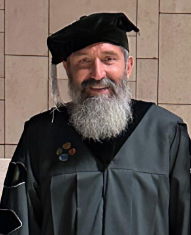
\includegraphics[scale=0.4]{Figures/Boffi.png}
				\begin{center}
					\small Daniele Boffi
				\end{center}
			\end{figure}
		\end{minipage}
	\end{frame}
	\begin{frame}{Fieldsplit Schur preconditioner}
		$\newline$
		$\newline$
		The previous set of equations can be written in matrix form as
		\vspace{-0.3cm}
		\begin{equation}
			\begin{bmatrix}
				A & B^T \\
				B & 0
			\end{bmatrix}
			\begin{bmatrix}\vec{u} \\p\end{bmatrix}=\begin{bmatrix}\vec{f} \\0\end{bmatrix}
		\end{equation}
		We choose as preconditioner the \textbf{fieldsplit Schur preconditioner}, i.e.
		\vspace{-0.3cm}
		\begin{equation}
			\begin{bmatrix}
				I & -\hat{A}^{-1} B^T\\
				0 & I
			\end{bmatrix}
			\begin{bmatrix}
				\hat{A}^{-1}& 0\\
				0 & \hat{S}^{-1}
			\end{bmatrix}
			\begin{bmatrix}
				I & 0\\
				-B\hat{A}^{-1} & I
			\end{bmatrix}
		\end{equation}
		where $S$ is the \textbf{Schur complement}, i.e. $S = -BA^{-1}B^T$.
		\lstinputlisting[language=python, firstline=18, lastline=21]{Examples/solvers.py}
	\end{frame}
	\begin{frame}
		\frametitle{Fieldsplit Schur preconditioner -- Mass matrix}
		$\newline$
		$\newline$
		Thanks to the inf-sup condition we can prove that the Schur complement is spectrally equivalent to the mass matrix, hence we can use as preconditioner:
		\begin{minipage}{0.7\textwidth}
			\vspace{-0.35cm}
			\begin{equation}
				\begin{bmatrix}
					I & -\hat{A}^{-1} B^T\\
					0 & I
				\end{bmatrix}
				\begin{bmatrix}
					\hat{A}^{-1}& 0\\
					0 & -\nu \hat{M}^{-1}
				\end{bmatrix}
				\begin{bmatrix}
					I & 0\\
					-B\hat{A}^{-1} & I
				\end{bmatrix}
			\end{equation}
			where $M$ is the mass matrix.
			\lstinputlisting[language=python,firstline=43,lastline=47]{Examples/multigrid.py}
		\end{minipage}
		\begin{minipage}{0.28\textwidth}
			\begin{figure}
				\centering
				\qquad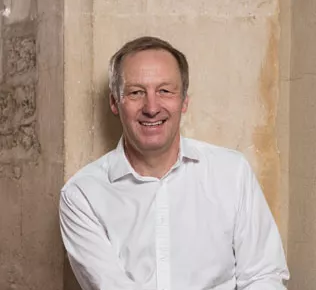
\includegraphics[scale=0.35]{Figures/Wathen.png}
				\begin{center}
					\small Andrew Wathen
				\end{center}
			\end{figure}
		\end{minipage}
	\end{frame}
	\begin{frame}{Multigrid on curved meshes}
		$\newline$
		ngsPETSc allows us to create a hierarchy of curved meshes for multigrid solvers.
		\lstinputlisting[language=python,firstline=19,lastline=21]{Examples/multigrid.py}
		We can than use a multigrid solver to compute $\hat{A}^{-1}$:
		\lstinputlisting[language=python,firstline=18,lastline=23]{Examples/solvers.py}
	\end{frame}
	\begin{frame}{Monolithic multigrid on curved meshes -- Coarse mesh}
		$\newline$
		We can also a monolithic multigrid solver for the Schur complement:
		\lstinputlisting[language=python,firstline=30,lastline=38]{Examples/solvers.py}
	\end{frame}
	\begin{frame}{Monolithic multigrid on curved meshes -- Fine mesh}
		$\newline$
		\lstinputlisting[language=python,firstline=43,lastline=53]{Examples/solvers.py}
	\end{frame}
	\begin{frame}{Navier-Stokes flow}
		A more interesting example is the Navier-Stokes flow, which is a non-linear problem.
		In particular, we will consider the problem of finding $(\vec{u},p) \in H^1(\Omega)^2\times L^2_0(\Omega)$ such that
		\begin{align*}
			\int_\Omega \partial_t \vec{u} \cdot \vec{v} + \int_\Omega(\nabla \vec{u})\vec{u}\cdot\vec{v}+\nu\int_{\Omega} \nabla \vec{u} : \nabla \vec{v} - \int_{\Omega} p \nabla \cdot \vec{v} &= \int_{\Omega} \vec{f} \cdot \vec{v}\\
			\int_{\Omega} q \nabla \cdot \vec{u} &= 0
		\end{align*}
		for all $(\vec{v},q) \in H^1(\Omega)^2\times L^2_0(\Omega)$.
	\end{frame}
	\begin{frame}{Navier-Stokes flow -- Augmented Lagrangian}
		$\newline$
		We consider an augmented Lagrangian formulation for the discrete problem, i.e. find $(\vec{u}_h,p_h) \in V_h \times Q_h$ such that
		\begin{align*}
			(\partial_t\vec{u},\vec{v})_0 + (\nabla \vec{u}\vec{u},\vec{v})_0 &+ \nu(\nabla \vec{u},\nabla \vec{v})_0 \\
			 & - (p,\nabla \cdot \vec{v})_0 + \frac{\gamma}{2}(\nabla \cdot \vec{u},\nabla \cdot \vec{v})_0 &= (\vec{f},\vec{v})_0\\
		\end{align*}
		and verifying the weak divergence free constraint $(\nabla \cdot \vec{u},q)_0 = 0$, for all $(\vec{v},q) \in V_h \times Q_h$.
	\end{frame}
	\begin{frame}
		\frametitle{Navier-Stokes flow -- Fieldsplit Schour preconditioner}
		$\newline$
		$\newline$
		The linearized version of the Navier-Stokes equations can be written in matrix form as 
		\vspace{-0.3cm}
		\begin{equation}
			\begin{bmatrix}
				A+\gamma B^TWB& B^T \\
				B & 0
			\end{bmatrix}
			\begin{bmatrix}\vec{u} \\p\end{bmatrix}=\begin{bmatrix}\vec{f} \\0\end{bmatrix}
		\end{equation}
		We choose as preconditioner the \textbf{fieldsplit Schur preconditioner}, i.e.
		\vspace{-0.3cm}
		\begin{equation}
			\begin{bmatrix}
				I & -\hat{A}_\gamma^{-1} B^T\\
				0 & I
			\end{bmatrix}
			\begin{bmatrix}
				\hat{A}_\gamma^{-1}& 0\\
				0 & \hat{S}_\gamma^{-1}
			\end{bmatrix}
			\begin{bmatrix}
				I & 0\\
				-BA_\gamma^{-1} & I
			\end{bmatrix}
		\end{equation}
		\begin{equation}
			A_\gamma = A+\gamma B^TWB 	\qquad  S_\gamma = -BA_\gamma^{-1}B^T.
		\end{equation}
		In this case, we notice that independently of the Reynolds numbers $S_\gamma\sim - (\nu+\gamma)^{-1} M$.
	\end{frame}
	\begin{frame}{Navier-Stokes flow -- Augmented Lagrangian}
		$\newline$
		\begin{itemize}
			\item [\color{oxfordblue}$\blacktriangleright$] The augmented Lagrangian term helps enforce the divergence-free constraint, and makes the scheme pressure robuts.
			\item [\color{oxfordblue}$\blacktriangleright$] We can use as preconditioner
			\begin{equation}
				\begin{bmatrix}
					I & -\hat{A}_\gamma^{-1} B^T\\
					0 & I
				\end{bmatrix}
				\begin{bmatrix}
					\hat{A}_\gamma^{-1}& 0\\
					0 & -(\nu+\gamma)M^{-1}
				\end{bmatrix}
				\begin{bmatrix}
					I & 0\\
					-BA_\gamma^{-1} & I
				\end{bmatrix}
			\end{equation}
			\item[\color{oxfordblue}$\blacktriangleright$] How do we compute $\hat{A}_\gamma^{-1}$ efficiently ? Can we adopt a multigrid approach ?
		\end{itemize}
	\end{frame}
	\begin{frame}
		\frametitle{Subspace correction methods for nearly singular
problems}
		$\newline$
		$\newline$
		To compute $\hat{A}_\gamma^{-1}$ we can use a subspace correction method.
		We decompose the space $V_h$ as follows:
		\vspace{-0.3cm}
		\begin{equation}
			V_h = \sum_{i=1} V_i.
		\end{equation}
		We consider a coarse space $V_H$ and the projection and injection operators:
		\vspace{-0.3cm}
		\begin{equation}
			P_H : V_H \rightarrow V_h, \qquad I : V_h \rightarrow V_i.
		\end{equation}
		We then consider as smoother the additive Schwarz preconditioner defined as:
		\begin{equation}
			\hat{A}_\gamma^{-1} = P_H A_{\gamma,H}^{-1} P_H^T + \sum_{i=1} I_i A_{\gamma,i}^{-1} I_i^T.
		\end{equation}
	\end{frame}
	\begin{frame}
		\frametitle{Subspace correction methods for nearly singular
problems}
		$\newline$
		\begin{block}{Robust relaxetion}
			We need the discrete kernel,
			\vspace{-0.3cm}
			\begin{equation}
				\mathbb{K}_h =  \{\vec{v} \in V_h : B\vec{v} = 0\},
			\end{equation}
			to decompose in a \textbf{stable} way as follows:
			\vspace{-0.3cm}
			\begin{equation}
				\mathbb{K}_h = \sum_{i=1} \mathbb{K}_h\cap V_i.
			\end{equation}
		\end{block}
	\end{frame}
	\begin{frame}[fragile]
		\frametitle{Robust relaxation -- Hood--Taylor}
		\begin{equation*}
			\begin{tikzcd}[row sep=huge]
			0 \arrow[r,""] & \Big[H^2(\Omega)\Big]^2 \arrow[r,"\curl"] \arrow[d]& \Big[H^1_0(\Omega)\Big]^2 \arrow[r,"\div"] \arrow[d]& L^2_0(\Omega) \arrow[r,""]\arrow[d] & 0\\
			0 \arrow[r,""] & \Big[\mathbb{P}^4(\mathcal{T}_h)\Big]^2 \arrow[r,"\curl"] & \Big[\mathbb{P}^3(\mathcal{T}_h)\Big]^2 \arrow[r,"\div"] & \mathbb{P}^2_{disc}(\mathcal{T}_h) \arrow[r,""] & 0\\
			\end{tikzcd}
		\end{equation*}
		\vspace{-2cm}
		\begin{figure}[h]
			\centering
			\hspace{1cm}\scalebox{0.45}{\tikzfig{Figures/DoF}}
		\end{figure}
	\end{frame}
	\begin{frame}
		\frametitle{Robust prolongation -- Hood--Taylor}
		$\newline$
		\begin{block}{Robust relaxetion}
			If the space pair $(V_h,Q_h)$ is inf-sup stable and the mesh we have a robust prolongation operator defined by:
			\begin{equation}
				\tilde P_H \vec{u}_H - \tilde{\vec{u}}_h = \vec{u}_H-\tilde{\vec{u}}_h,
			\end{equation}
			where
			\begin{equation}
				a_{\gamma}(\tilde{\vec{u}}_h,\tilde{\vec{v}}_h) = \gamma(\nabla \cdot \tilde{\vec{u}}_h,\nabla \cdot \tilde{\vec{v}}_h)_{\pi_{Q_h}\pi{Q_h}^T} \quad \forall \tilde{\vec{v}}_h \in \tilde{V}_h,
			\end{equation}
			where $\pi_{Q_h}$ is the $L^2$ projection onto $Q_h$ and $\tilde{V}_h$ is the space of discrete velocity vanishing at the boundary of the coarse cells.
		\end{block}
	\end{frame}
	\begin{frame}
		\frametitle{Numerical Simulation}
		\begin{figure}
			\centering
			\scalebox{0.2}{\animategraphics[loop,autoplay]{12}{Figures/NS/Velocity.}{0000}{0158}}
		\end{figure}
	\end{frame}
\end{document}


\pgfdeclareimage[width=\paperwidth]{titlebackground}{Images/title-slide-background.png}
\setbeamerfont{subtitle}{size=\tiny}
\setbeamertemplate{endpage}{
	\begin{picture}(0,0)
		\scalebox{1.01}{
		\put(-28.5,-163){%
			\pgfuseimage{titlebackground}
		}
		}
		\put(0,-115){%
			\begin{minipage}[b][4.5cm][t]{0.5\textwidth}
				\color{white}
				\usebeamerfont{title}
				{\textbf{Thank Your} \\ \textbf{For You Attention !}}
			\end{minipage}
		}
	\end{picture}
}
\setbeamertemplate{title page}{
	\begin{picture}(0,0)
		\scalebox{1.01}{
			\put(-28.5,-163){%
				\pgfuseimage{titlebackground}
			}
		}
		\put(0,-60){%
			\begin{minipage}[b][4.5cm][t]{0.7\textwidth}
				\color{white}
				\usebeamerfont{title}
				{\inserttitle\\[0.9cm]}
				\usebeamerfont{subtitle}
				{\insertauthor\par}
				{\insertinstitute\\[0.3cm]}
				{\insertdate}
			\end{minipage}
		}
	\end{picture}
}


%% General slide formatting %%

\definecolor{oxfordblue}{RGB}{4,30,66}
\definecolor{oxfordred}{RGB}{207,48,42}

\pgfdeclareimage[width=0.9cm]{oxfordlogo}{Images/oxford-logo.png}
\pgfdeclareimage[width=1cm]{mathslogo}{Images/mathematics-logo.png}
\pgfdeclareimage[width=1.2cm]{ngslogo}{Images/ngs-logo.png}
\pgfdeclareimage[width=1.2cm]{petsclogo}{Images/petsc-logo.png}
\pgfdeclareimage[width=1.2cm]{firedrakelogo}{Images/firedrake-logo.png}

\setbeamertemplate{headline}
{%
	\begin{picture}(0,0)
		\put(314,-50){%
			\pgfuseimage{oxfordlogo}
		}
		\put(20,-55){%
			\rule{320pt}{0.4pt}
		}
	\end{picture}
}
\def\ngshead{
	\begin{picture}(0,0)
		\put(278,0){%
			\pgfuseimage{ngslogo}
		}
		\put(-8,-5){%
			\rule{325pt}{0.4pt}
		}
	\end{picture}
}
\def\petschead{
	\begin{picture}(0,0)
		\put(278,0){%
			\pgfuseimage{petsclogo}
		}
		\put(-8,-5){%
			\rule{325pt}{0.4pt}
		}
	\end{picture}
}
\def\firedrakehead{
	\begin{picture}(0,0)
		\put(278,0){%
			\pgfuseimage{firedrakelogo}
		}
		\put(-8,-5){%
			\rule{325pt}{0.4pt}
		}
	\end{picture}
}
\setbeamertemplate{frametitle}
{%
	\begin{picture}(0,0)
		\put(-8,-20){%
			\normalsize\textbf{\color{oxfordblue}\insertframetitle}
		}
		\put(-8,-32){%
			\normalsize\textbf{\color{oxfordblue}\insertframesubtitle}
		}
	\end{picture}
}

\setbeamertemplate{footline}
{%
	\begin{picture}(0,0)
		\put(20,30){%
			\rule{320pt}{0.4pt}
		}
		\put(20,14){%
			\pgfuseimage{mathslogo}
		}
		\put(100,14){%
			\color{oxfordblue}\insertshortdate
		}
		\put(160,14){%
			\color{oxfordblue}\insertshorttitle
		}
		\put(337,14){%
			\color{oxfordblue}\insertframenumber
		}
	\end{picture}%
}
\def\footer{
	\begin{picture}(0,0)
		\put(-308,-75){%
			\rule{325pt}{0.4pt}
		}
		\put(-308,-91){%
			\pgfuseimage{mathslogo}
		}
		\put(-228,-91){%
			\color{oxfordblue}\tiny\insertshortdate
		}
		\put(-168,-91){%
			\color{oxfordblue}\tiny\insertshorttitle
		}
		\put(9,-91){%
			\color{oxfordblue}\tiny\insertframenumber
		}
	\end{picture}
}

\setbeamercolor{block title}{bg=oxfordblue!30,fg=black}
\setbeamercolor{palette primary}{bg=oxfordblue,fg=white}

\definecolor{codegreen}{rgb}{0,0.6,0}
\definecolor{codegray}{rgb}{0.5,0.5,0.5}
\definecolor{codepurple}{rgb}{0.58,0,0.82}
\definecolor{backcolour}{rgb}{0.95,0.95,0.92}

\lstdefinestyle{mystyle}{
	%backgroundcolor=\color{backcolour},   
	commentstyle=\color{codegray},
	keywordstyle=\color{oxfordblue},
	numberstyle=\tiny\color{codegray},
	stringstyle=\color{codegreen},
	basicstyle=\ttfamily\footnotesize,
	breakatwhitespace=false,         
	breaklines=true,                 
	captionpos=b,                    
	keepspaces=true,                 
	numbers=left,                    
	numbersep=5pt,                  
	showspaces=false,                
	showstringspaces=false,
	showtabs=false,                  
	tabsize=2
}
\AtBeginSection[]{
  \begin{frame}
  \vfill
  \centering
  \begin{beamercolorbox}[sep=8pt,center,shadow=true,rounded=true]{title}
    \usebeamerfont{title}\insertsectionhead\par%
  \end{beamercolorbox}
  \vfill
  \end{frame}
}

\lstset{style=mystyle}

%% Information (author, title, etc.) %%
\title[ngsPETSc]{ngsPETSc: NETGEN meets PETSc} % short title for footer
\author%
{%
	\sc{P.~E.~Farrell}*, \sc{S.~Zampini$\dag$}, \underline{\sc{U.~Zerbinati}}*\\
}
\institute%
{%
	* \textit{Mathematical Institute}\\
	\;\textit{University of Oxford}\\
	$\newline$
	$\dag$ \textit{Extreme Computing Research Center}\\
	\;\textit{King Abdullah University of Science and Technology}\\	
}

\date[\textbf{DD28}]{28 International Conference on Domain Decomposition Methods, 29th Jannuary 2024, KAUST} % short date for footer



%% Content of slides %%

\begin{document}
	\begin{frame}[plain]
		\titlepage
	\end{frame}
	\begin{frame}[plain]
		\frametitle{NETGEN}
		\ngshead
		$\newline$
		$\newline$
		NETGEN is an advancing front 2D/3D-mesh generator, with many interesting features.
		$\newline$
		$\newline$
		\begin{minipage}{0.58\textwidth}
			\begin{itemize}
				\item[\color{oxfordblue}$\blacktriangleright$] The geometry we intend to mesh can be described by \textbf{Constructive Solid Geometry} (CSG), in particular we can use \textbf{Opencascade} to describe our geometry.
				\item[\color{oxfordblue}$\blacktriangleright$] It is able to construct isoparametric meshes, which conform to the geometry.
			\end{itemize}
		\end{minipage}
		\qquad
		\begin{minipage}{0.3\textwidth}
			\begin{figure}
				\centering
				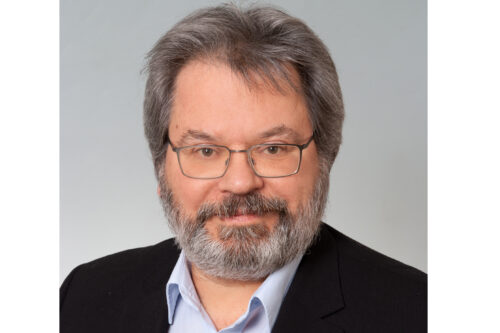
\includegraphics[scale=1.]{Figures/Schoeberl.jpg}
				\begin{center}
					\qquad\small Joachim Sc\"{o}berl
				\end{center}
			\end{figure}
			\vspace{0.3cm}
		\end{minipage}
	\end{frame}

	\begin{frame}[plain]
		$\newline$ 
		$\newline$ 
		\frametitle{PETSc}
		\petschead
		$\newline$
		$\newline$ 
		PETSc stands for Portable, Extensible Toolkit for Scientific Computation, is a library for the scalable (parallel) solution of scientific applications modeled by partial differential equations (PDEs).
		$\newline$
		\begin{minipage}{0.58\textwidth}
			\begin{itemize}
				\item[\color{oxfordblue}$\blacktriangleright$] \textbf{PETSc KSP} provides access to extremly efficent Krylov solvers.
				\item[\color{oxfordblue}$\blacktriangleright$] \textbf{PETSc SNES} provides access to extremly efficent non-linear solvers, with line-searching and trust region capabilities.
			\end{itemize}
		\end{minipage}
		\qquad
		\begin{minipage}{0.3\textwidth}
			\begin{figure}
				\centering
				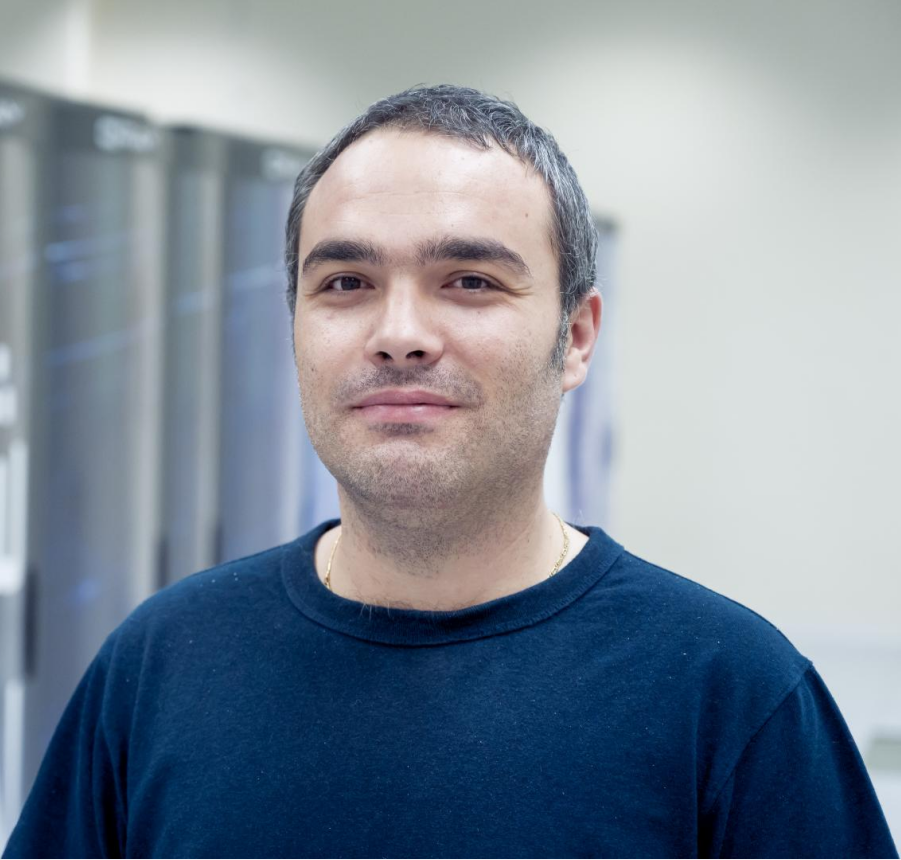
\includegraphics[scale=0.15]{Figures/Zampini.png}
				\begin{center}
					\;\;\small Stefano Zampini
				\end{center}
			\end{figure}
		\end{minipage}
		\vspace{3cm}
	\end{frame}
	\begin{frame}
		\frametitle{ngsPETSc -- NETGEN/NGSolve}
		$\newline$
		\textbf{ngsPETSc} is an interface between NETGEN/NGSolve and \textbf{PETSc}. In particular, \textbf{ngsPETSc} provides new capabilities to \textbf{NETGEN}/\textbf{NGSolve} such as:
		$\newline$
		\begin{itemize}
			\item[\color{oxfordblue}$\blacktriangleright$] Access to all linear solver capabilities of \textbf{KSP}.
			\item[\color{oxfordblue}$\blacktriangleright$] Access to all preconditioning capabilities of \textbf{PC}.
			\item[\color{oxfordblue}$\blacktriangleright$] Access to all non-linear solver capabilities of \textbf{SNES}.
			\item[\color{oxfordblue}$\blacktriangleright$] Access to all mesh refinement capabilities of \textbf{DMPLEX}.
		\end{itemize}
	\end{frame}
	\begin{frame}[plain]
		$\newline$ 
		\petschead
		\frametitle{PETSc DMPlex}
		$\newline$ 
		$\newline$
		\begin{minipage}{0.58\textwidth}
			\textbf{PETSc DMPlex} handles unstructured grids using the generic \textbf{PETSc} interface for hierarchy and multi-physics. 
			$\newline$
			\begin{itemize}
				\item[\color{oxfordblue}$\blacktriangleright$] \textbf{PETSc DMPlex} provides a wide variety of primitive mesh operations such as: \textit{meet}, \textit{clousre}, \textit{cone}, etc
				\item[\color{oxfordblue}$\blacktriangleright$] \textbf{PETSc DMPlex} provides a wide variety of mesh refinement operations such as: \textit{unifrom refinement}, \textit{Alfeld refinement}, \textit{box refinement}, etc
			\end{itemize}
		\end{minipage}
		\qquad
		\begin{minipage}{0.33\textwidth}
			\begin{figure}
				\centering
				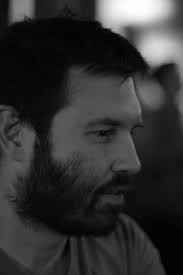
\includegraphics[scale=0.5]{Figures/Kneply.jpeg}
				\begin{center}
					\hspace{0.5cm}\small Matthew G.~Knepley
				\end{center}
			\end{figure}
		\end{minipage}
	\end{frame}
	\begin{frame}[plain]
		\firedrakehead
		$\newline$
		$\newline$
		\textbf{Firedrake} is an automated system for the solution of partial differential equations using the finite element method (FEM).
		$\newline$
		$\newline$
		\begin{minipage}{0.58\textwidth}
			\begin{itemize}
				\item[\color{oxfordblue}$\blacktriangleright$] Variational formulation can be easily defined using the \textbf{UFL} language.
				\item[\color{oxfordblue}$\blacktriangleright$] Wide class of finite elements are available, including $H(div)$, $H(curl)$, $H^1$ and $H^2$.
				\item[\color{oxfordblue}$\blacktriangleright$] Provides access to \textbf{PETSc} linear solvers and non-linear solvers.
			\end{itemize}
		\end{minipage}
		\qquad
		\begin{minipage}{0.3\textwidth}
			\begin{figure}
				\centering
				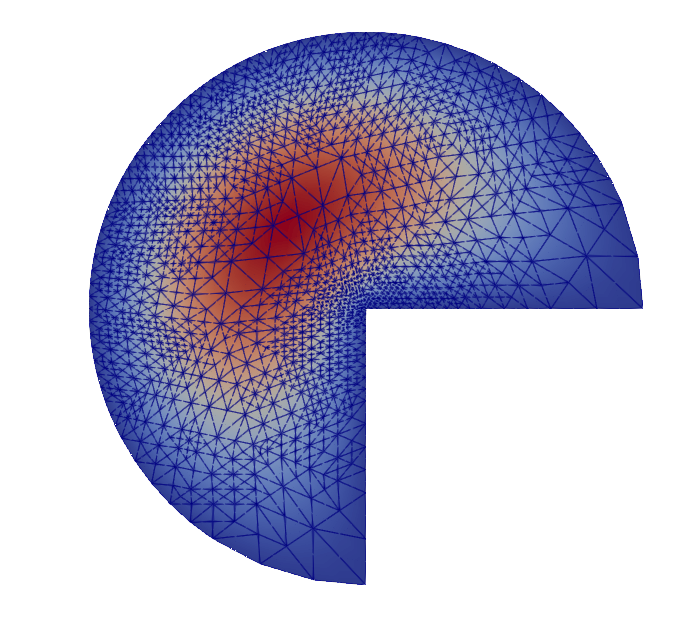
\includegraphics[scale=0.2]{Figures/Pacman.png}
			\end{figure}
			\vspace{0.3cm}
		\end{minipage}
	\end{frame}
	\begin{frame}
		\frametitle{ngsPETSc -- Firedrake}
		$\newline$
		\textbf{ngsPETSc} provides new capabilities to \textbf{Firedrake} such as:
		$\newline$
		\begin{itemize}
			\item[\color{oxfordblue}$\blacktriangleright$] Access to all Netgen generated linear meshes and high order meshes.
			\item[\color{oxfordblue}$\blacktriangleright$] Splits for macro elements, such as Alfeld splits and Powell-Sabin splits (even on curved geometries).
			\item[\color{oxfordblue}$\blacktriangleright$] Adaptive mesh refinement capabilities, that conform to the geometry.
			\item[\color{oxfordblue}$\blacktriangleright$] High order meshes hierarchy for multigrid solvers.
		\end{itemize}
	\end{frame}
	\begin{frame}{Examples -- Opencascade via NETGEN}
		\lstinputlisting[language=python,firstline=4,lastline=14]{Examples/occ.py}
	\end{frame}
	\begin{frame}{Examples -- Opencascade via NETGEN}
		$\newline$
		\lstinputlisting[language=python,firstline=15,lastline=17]{Examples/occ.py}
	\begin{figure}
			\centering
			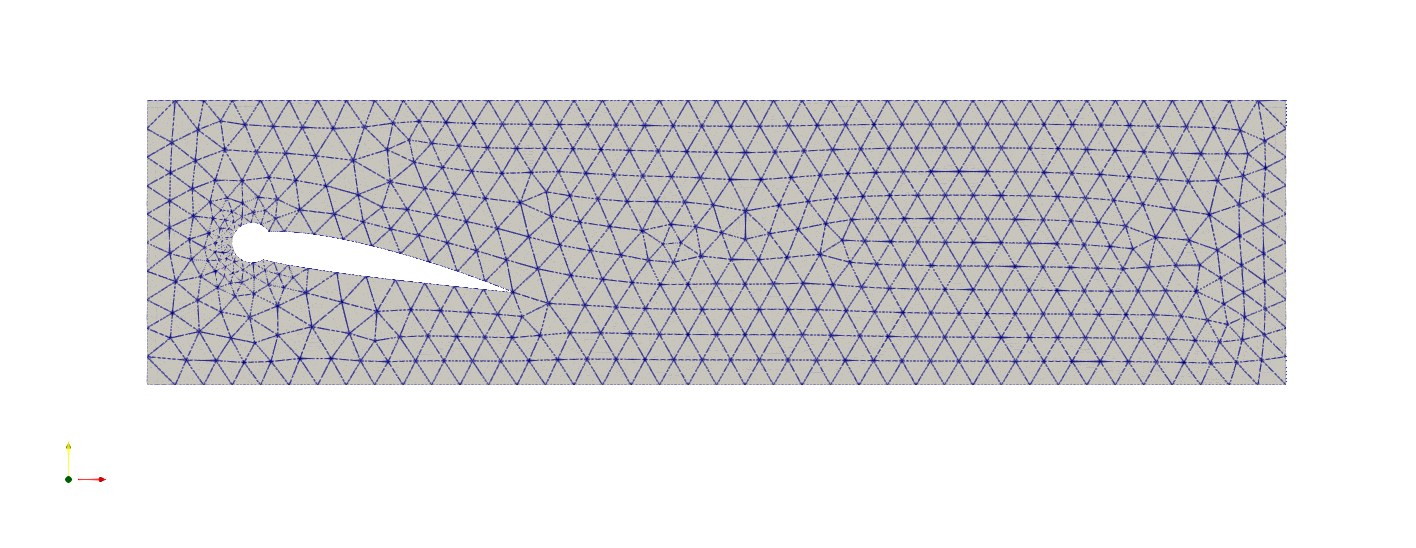
\includegraphics[scale=0.2]{Figures/nacaMesh.png}
		\end{figure}	
	\end{frame}
	\begin{frame}{Stokes flow -- Weak formulation}
		$\newline$
		Find $(\vec{u},p) \in V \times Q$ such that
		\begin{align*}
			\int_{\Omega} \nabla \vec{u} : \nabla \vec{v} - \int_{\Omega} p \nabla \cdot \vec{v} &= \int_{\Omega} \vec{f} \cdot \vec{v} \quad &\forall \vec{v} \in V \\
			\int_{\Omega} q \nabla \cdot \vec{u} &= 0 \quad &\forall q \in Q
		\end{align*}
		where $V$ and $Q$ are the velocity and pressure spaces respectively, i.e. $V = H^1_0(\Omega)^2$ and $Q = L^2_0(\Omega)$.
	\end{frame}
	\begin{frame}
		\frametitle{Stokes flow -- Inf-sup condition}
		$\newline$
		$\newline$
		We can also look for a discrete solution, i.e. find $(\vec{u}_h,p_h) \in V_h \times Q_h$ such that	
		\begin{minipage}{0.75\textwidth}
			\begin{gather}
				\nu\int_{\Omega} \nabla \vec{u} : \nabla \vec{v} - \int_{\Omega} p \nabla \cdot \vec{v} = \int_{\Omega} \vec{f} \cdot \vec{v}\\
				\int_{\Omega} q \nabla \cdot \vec{u} = 0
			\end{gather}
		for all $(\vec{v},q) \in V_h \times Q_h$.
		\begin{equation}
			\underset{q\in Q_h}{\inf} \underset{\vec{v}\in V_h}{\sup} \frac{\int_{\Omega} q \nabla \cdot \vec{v}}{\norm{q}_{L^2} \norm{\vec{v}}_{H^1}} \geq \beta > 0	
		\end{equation}
		\end{minipage}
		\begin{minipage}{0.2\textwidth}
			\begin{figure}
				\centering
				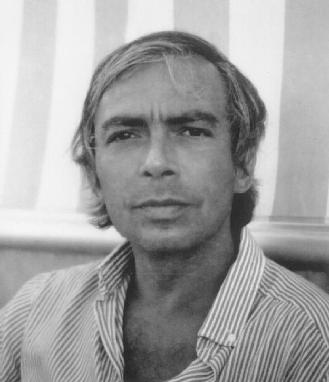
\includegraphics[scale=0.2]{Figures/Brezzi.jpg}
				\begin{center}
					\small Franco Brezzi
				\end{center}
			\end{figure}
		\end{minipage}
	\end{frame}
	\begin{frame}
		\frametitle{Stokes flow -- UFL}
		$\newline$
		\lstinputlisting[language=python,firstline=27,lastline=31]{Examples/scottVogelius.py}
	\end{frame}
	\begin{frame}
		\frametitle{Stokes flow -- Scott--Vogelius element}
		$\newline$
		$\newline$
		We can use the Scott--Vogelius pair, which is a mixed finite element of order $k$ for the velocity and order $k-1$ for the pressure.
		Such an element is inf-sup stable for $k \geq 2$, under certain assumptions on the mesh. Such pair is \textbf{divergence-free}.
		\begin{minipage}{0.75\textwidth}
			$\newline$	
			When $k=2$ we need \textbf{Alfeld splits}.
			\lstinputlisting[language=python,firstline=17,lastline=19]{Examples/scottVogelius.py}
			\lstinputlisting[language=python,firstline=24,lastline=26]{Examples/scottVogelius.py}
		\end{minipage}
		\begin{minipage}{0.2\textwidth}
			\begin{figure}
				\centering
				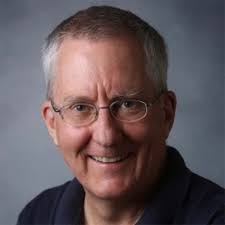
\includegraphics[scale=0.3]{Figures/Scott.jpeg}
				\begin{center}
					\small Ridgway Scott
				\end{center}
			\end{figure}
		\end{minipage}
	\end{frame}
	\begin{frame}
		\frametitle{Stokes flow -- Scott--Vogelius}
		$\newline$
		\lstinputlisting[language=python,firstline=38,lastline=41]{Examples/scottVogelius.py}
		\vspace{-1cm}
		\begin{figure}
			\centering
			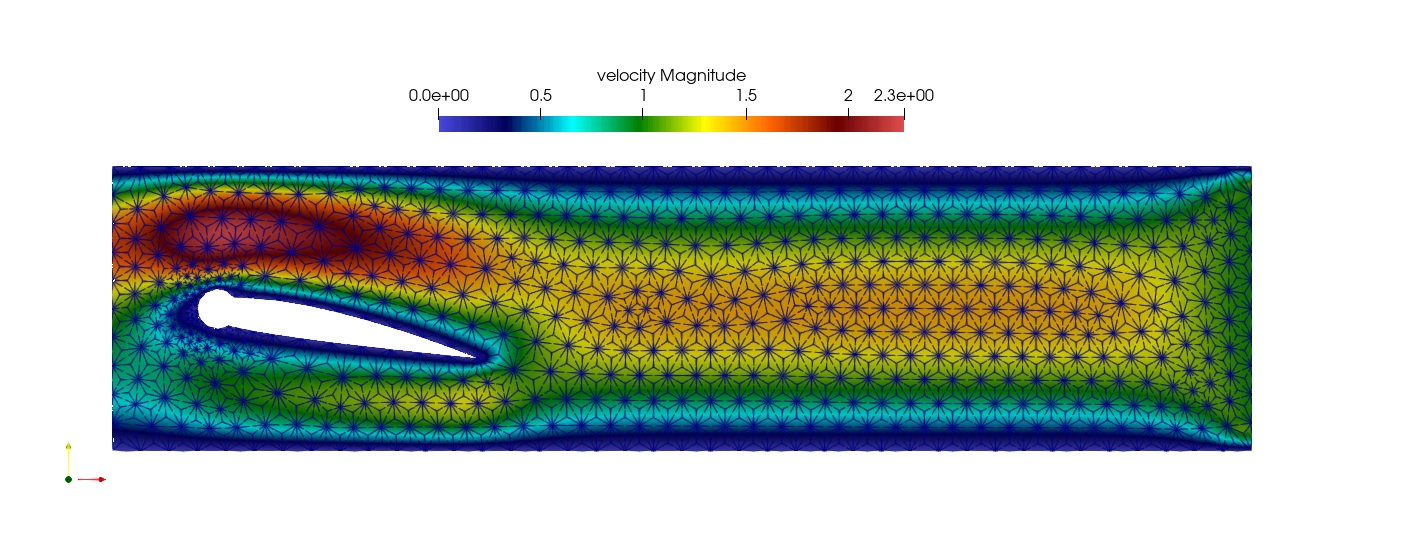
\includegraphics[scale=0.2]{Figures/scottVogelius.png}
		\end{figure}
	\end{frame}
	\begin{frame}
		\frametitle{Stokes flow -- Hood--Taylor element}
		$\newline$
		$\newline$
		Another element pair we will use is the Hood--Taylor pair, which has \textbf{no restrictions} on the mesh in two dimensions.
		$\newline$
		$\newline$
		\begin{minipage}{0.8\textwidth}
			\lstinputlisting[language=python,firstline=24,lastline=26]{Examples/hoodTaylor.py}
			\textbf{We lose the point-wise divergence-free property!}
			This is not an issue because the same would happen for Scott-Vogelius on curved meshes.
		\end{minipage}
		\begin{minipage}{0.18\textwidth}
			\begin{figure}
				\centering
				\qquad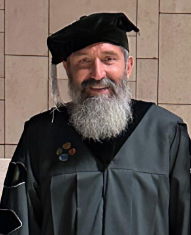
\includegraphics[scale=0.4]{Figures/Boffi.png}
				\begin{center}
					\small Daniele Boffi
				\end{center}
			\end{figure}
		\end{minipage}
	\end{frame}
	\begin{frame}{Fieldsplit Schur preconditioner}
		$\newline$
		$\newline$
		The previous set of equations can be written in matrix form as
		\vspace{-0.3cm}
		\begin{equation}
			\begin{bmatrix}
				A & B^T \\
				B & 0
			\end{bmatrix}
			\begin{bmatrix}\vec{u} \\p\end{bmatrix}=\begin{bmatrix}\vec{f} \\0\end{bmatrix}
		\end{equation}
		We choose as preconditioner the \textbf{fieldsplit Schur preconditioner}, i.e.
		\vspace{-0.3cm}
		\begin{equation}
			\begin{bmatrix}
				I & -\hat{A}^{-1} B^T\\
				0 & I
			\end{bmatrix}
			\begin{bmatrix}
				\hat{A}^{-1}& 0\\
				0 & \hat{S}^{-1}
			\end{bmatrix}
			\begin{bmatrix}
				I & 0\\
				-B\hat{A}^{-1} & I
			\end{bmatrix}
		\end{equation}
		where $S$ is the \textbf{Schur complement}, i.e. $S = -BA^{-1}B^T$.
		\lstinputlisting[language=python, firstline=18, lastline=21]{Examples/solvers.py}
	\end{frame}
	\begin{frame}
		\frametitle{Fieldsplit Schur preconditioner -- Mass matrix}
		$\newline$
		$\newline$
		Thanks to the inf-sup condition we can prove that the Schur complement is spectrally equivalent to the mass matrix, hence we can use as preconditioner:
		\begin{minipage}{0.7\textwidth}
			\vspace{-0.35cm}
			\begin{equation}
				\begin{bmatrix}
					I & -\hat{A}^{-1} B^T\\
					0 & I
				\end{bmatrix}
				\begin{bmatrix}
					\hat{A}^{-1}& 0\\
					0 & -\nu \hat{M}^{-1}
				\end{bmatrix}
				\begin{bmatrix}
					I & 0\\
					-B\hat{A}^{-1} & I
				\end{bmatrix}
			\end{equation}
			where $M$ is the mass matrix.
			\lstinputlisting[language=python,firstline=43,lastline=47]{Examples/multigrid.py}
		\end{minipage}
		\begin{minipage}{0.28\textwidth}
			\begin{figure}
				\centering
				\qquad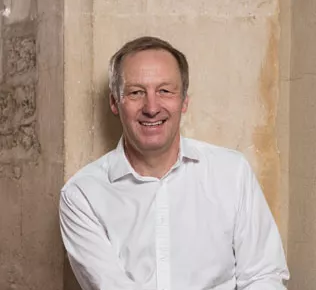
\includegraphics[scale=0.35]{Figures/Wathen.png}
				\begin{center}
					\small Andrew Wathen
				\end{center}
			\end{figure}
		\end{minipage}
	\end{frame}
	\begin{frame}{Multigrid on curved meshes}
		$\newline$
		ngsPETSc allows us to create a hierarchy of curved meshes for multigrid solvers.
		\lstinputlisting[language=python,firstline=19,lastline=21]{Examples/multigrid.py}
		We can than use a multigrid solver to compute $\hat{A}^{-1}$:
		\lstinputlisting[language=python,firstline=18,lastline=23]{Examples/solvers.py}
	\end{frame}
	\begin{frame}{Monolithic multigrid on curved meshes -- Coarse mesh}
		$\newline$
		We can also a monolithic multigrid solver for the Schur complement:
		\lstinputlisting[language=python,firstline=30,lastline=38]{Examples/solvers.py}
	\end{frame}
	\begin{frame}{Monolithic multigrid on curved meshes -- Fine mesh}
		$\newline$
		\lstinputlisting[language=python,firstline=43,lastline=53]{Examples/solvers.py}
	\end{frame}
	\begin{frame}{Navier-Stokes flow}
		A more interesting example is the Navier-Stokes flow, which is a non-linear problem.
		In particular, we will consider the problem of finding $(\vec{u},p) \in H^1(\Omega)^2\times L^2_0(\Omega)$ such that
		\begin{align*}
			\int_\Omega \partial_t \vec{u} \cdot \vec{v} + \int_\Omega(\nabla \vec{u})\vec{u}\cdot\vec{v}+\nu\int_{\Omega} \nabla \vec{u} : \nabla \vec{v} - \int_{\Omega} p \nabla \cdot \vec{v} &= \int_{\Omega} \vec{f} \cdot \vec{v}\\
			\int_{\Omega} q \nabla \cdot \vec{u} &= 0
		\end{align*}
		for all $(\vec{v},q) \in H^1(\Omega)^2\times L^2_0(\Omega)$.
	\end{frame}
	\begin{frame}{Navier-Stokes flow -- Augmented Lagrangian}
		$\newline$
		We consider an augmented Lagrangian formulation for the discrete problem, i.e. find $(\vec{u}_h,p_h) \in V_h \times Q_h$ such that
		\begin{align*}
			(\partial_t\vec{u},\vec{v})_0 + (\nabla \vec{u}\vec{u},\vec{v})_0 &+ \nu(\nabla \vec{u},\nabla \vec{v})_0 \\
			 & - (p,\nabla \cdot \vec{v})_0 + \frac{\gamma}{2}(\nabla \cdot \vec{u},\nabla \cdot \vec{v})_0 &= (\vec{f},\vec{v})_0\\
		\end{align*}
		and verifying the weak divergence free constraint $(\nabla \cdot \vec{u},q)_0 = 0$, for all $(\vec{v},q) \in V_h \times Q_h$.
	\end{frame}
	\begin{frame}
		\frametitle{Navier-Stokes flow -- Fieldsplit Schour preconditioner}
		$\newline$
		$\newline$
		The linearized version of the Navier-Stokes equations can be written in matrix form as 
		\vspace{-0.3cm}
		\begin{equation}
			\begin{bmatrix}
				A+\gamma B^TWB& B^T \\
				B & 0
			\end{bmatrix}
			\begin{bmatrix}\vec{u} \\p\end{bmatrix}=\begin{bmatrix}\vec{f} \\0\end{bmatrix}
		\end{equation}
		We choose as preconditioner the \textbf{fieldsplit Schur preconditioner}, i.e.
		\vspace{-0.3cm}
		\begin{equation}
			\begin{bmatrix}
				I & -\hat{A}_\gamma^{-1} B^T\\
				0 & I
			\end{bmatrix}
			\begin{bmatrix}
				\hat{A}_\gamma^{-1}& 0\\
				0 & \hat{S}_\gamma^{-1}
			\end{bmatrix}
			\begin{bmatrix}
				I & 0\\
				-BA_\gamma^{-1} & I
			\end{bmatrix}
		\end{equation}
		\begin{equation}
			A_\gamma = A+\gamma B^TWB 	\qquad  S_\gamma = -BA_\gamma^{-1}B^T.
		\end{equation}
		In this case, we notice that independently of the Reynolds numbers $S_\gamma\sim - (\nu+\gamma)^{-1} M$.
	\end{frame}
	\begin{frame}{Navier-Stokes flow -- Augmented Lagrangian}
		$\newline$
		\begin{itemize}
			\item [\color{oxfordblue}$\blacktriangleright$] The augmented Lagrangian term helps enforce the divergence-free constraint, and makes the scheme pressure robuts.
			\item [\color{oxfordblue}$\blacktriangleright$] We can use as preconditioner
			\begin{equation}
				\begin{bmatrix}
					I & -\hat{A}_\gamma^{-1} B^T\\
					0 & I
				\end{bmatrix}
				\begin{bmatrix}
					\hat{A}_\gamma^{-1}& 0\\
					0 & -(\nu+\gamma)M^{-1}
				\end{bmatrix}
				\begin{bmatrix}
					I & 0\\
					-BA_\gamma^{-1} & I
				\end{bmatrix}
			\end{equation}
			\item[\color{oxfordblue}$\blacktriangleright$] How do we compute $\hat{A}_\gamma^{-1}$ efficiently ? Can we adopt a multigrid approach ?
		\end{itemize}
	\end{frame}
	\begin{frame}
		\frametitle{Subspace correction methods for nearly singular
problems}
		$\newline$
		$\newline$
		To compute $\hat{A}_\gamma^{-1}$ we can use a subspace correction method.
		We decompose the space $V_h$ as follows:
		\vspace{-0.3cm}
		\begin{equation}
			V_h = \sum_{i=1} V_i.
		\end{equation}
		We consider a coarse space $V_H$ and the projection and injection operators:
		\vspace{-0.3cm}
		\begin{equation}
			P_H : V_H \rightarrow V_h, \qquad I : V_h \rightarrow V_i.
		\end{equation}
		We then consider as smoother the additive Schwarz preconditioner defined as:
		\begin{equation}
			\hat{A}_\gamma^{-1} = P_H A_{\gamma,H}^{-1} P_H^T + \sum_{i=1} I_i A_{\gamma,i}^{-1} I_i^T.
		\end{equation}
	\end{frame}
	\begin{frame}
		\frametitle{Subspace correction methods for nearly singular
problems}
		$\newline$
		\begin{block}{Robust relaxetion}
			We need the discrete kernel,
			\vspace{-0.3cm}
			\begin{equation}
				\mathbb{K}_h =  \{\vec{v} \in V_h : B\vec{v} = 0\},
			\end{equation}
			to decompose in a \textbf{stable} way as follows:
			\vspace{-0.3cm}
			\begin{equation}
				\mathbb{K}_h = \sum_{i=1} \mathbb{K}_h\cap V_i.
			\end{equation}
		\end{block}
	\end{frame}
	\begin{frame}[fragile]
		\frametitle{Robust relaxation -- Hood--Taylor}
		\begin{equation*}
			\begin{tikzcd}[row sep=huge]
			0 \arrow[r,""] & \Big[H^2(\Omega)\Big]^2 \arrow[r,"\curl"] \arrow[d]& \Big[H^1_0(\Omega)\Big]^2 \arrow[r,"\div"] \arrow[d]& L^2_0(\Omega) \arrow[r,""]\arrow[d] & 0\\
			0 \arrow[r,""] & \Big[\mathbb{P}^4(\mathcal{T}_h)\Big]^2 \arrow[r,"\curl"] & \Big[\mathbb{P}^3(\mathcal{T}_h)\Big]^2 \arrow[r,"\div"] & \mathbb{P}^2_{disc}(\mathcal{T}_h) \arrow[r,""] & 0\\
			\end{tikzcd}
		\end{equation*}
		\vspace{-2cm}
		\begin{figure}[h]
			\centering
			\hspace{1cm}\scalebox{0.45}{\tikzfig{Figures/DoF}}
		\end{figure}
	\end{frame}
	\begin{frame}
		\frametitle{Robust prolongation -- Hood--Taylor}
		$\newline$
		\begin{block}{Robust relaxetion}
			If the space pair $(V_h,Q_h)$ is inf-sup stable and the mesh we have a robust prolongation operator defined by:
			\begin{equation}
				\tilde P_H \vec{u}_H - \tilde{\vec{u}}_h = \vec{u}_H-\tilde{\vec{u}}_h,
			\end{equation}
			where
			\begin{equation}
				a_{\gamma}(\tilde{\vec{u}}_h,\tilde{\vec{v}}_h) = \gamma(\nabla \cdot \tilde{\vec{u}}_h,\nabla \cdot \tilde{\vec{v}}_h)_{\pi_{Q_h}\pi{Q_h}^T} \quad \forall \tilde{\vec{v}}_h \in \tilde{V}_h,
			\end{equation}
			where $\pi_{Q_h}$ is the $L^2$ projection onto $Q_h$ and $\tilde{V}_h$ is the space of discrete velocity vanishing at the boundary of the coarse cells.
		\end{block}
	\end{frame}
	\begin{frame}
		\frametitle{Numerical Simulation}
		\begin{figure}
			\centering
			\scalebox{0.2}{\animategraphics[loop,autoplay]{12}{Figures/NS/Velocity.}{0000}{0158}}
		\end{figure}
	\end{frame}
\end{document}


\pgfdeclareimage[width=\paperwidth]{titlebackground}{Images/title-slide-background.png}
\setbeamerfont{subtitle}{size=\tiny}
\setbeamertemplate{endpage}{
	\begin{picture}(0,0)
		\scalebox{1.01}{
		\put(-28.5,-163){%
			\pgfuseimage{titlebackground}
		}
		}
		\put(0,-115){%
			\begin{minipage}[b][4.5cm][t]{0.5\textwidth}
				\color{white}
				\usebeamerfont{title}
				{\textbf{Thank Your} \\ \textbf{For You Attention !}}
			\end{minipage}
		}
	\end{picture}
}
\setbeamertemplate{title page}{
	\begin{picture}(0,0)
		\scalebox{1.01}{
			\put(-28.5,-163){%
				\pgfuseimage{titlebackground}
			}
		}
		\put(0,-60){%
			\begin{minipage}[b][4.5cm][t]{0.7\textwidth}
				\color{white}
				\usebeamerfont{title}
				{\inserttitle\\[0.9cm]}
				\usebeamerfont{subtitle}
				{\insertauthor\par}
				{\insertinstitute\\[0.3cm]}
				{\insertdate}
			\end{minipage}
		}
	\end{picture}
}


%% General slide formatting %%

\definecolor{oxfordblue}{RGB}{4,30,66}
\definecolor{oxfordred}{RGB}{207,48,42}

\pgfdeclareimage[width=0.9cm]{oxfordlogo}{Images/oxford-logo.png}
\pgfdeclareimage[width=1cm]{mathslogo}{Images/mathematics-logo.png}
\pgfdeclareimage[width=1.2cm]{ngslogo}{Images/ngs-logo.png}
\pgfdeclareimage[width=1.2cm]{petsclogo}{Images/petsc-logo.png}
\pgfdeclareimage[width=1.2cm]{firedrakelogo}{Images/firedrake-logo.png}

\setbeamertemplate{headline}
{%
	\begin{picture}(0,0)
		\put(314,-50){%
			\pgfuseimage{oxfordlogo}
		}
		\put(20,-55){%
			\rule{320pt}{0.4pt}
		}
	\end{picture}
}
\def\ngshead{
	\begin{picture}(0,0)
		\put(278,0){%
			\pgfuseimage{ngslogo}
		}
		\put(-8,-5){%
			\rule{325pt}{0.4pt}
		}
	\end{picture}
}
\def\petschead{
	\begin{picture}(0,0)
		\put(278,0){%
			\pgfuseimage{petsclogo}
		}
		\put(-8,-5){%
			\rule{325pt}{0.4pt}
		}
	\end{picture}
}
\def\firedrakehead{
	\begin{picture}(0,0)
		\put(278,0){%
			\pgfuseimage{firedrakelogo}
		}
		\put(-8,-5){%
			\rule{325pt}{0.4pt}
		}
	\end{picture}
}
\setbeamertemplate{frametitle}
{%
	\begin{picture}(0,0)
		\put(-8,-20){%
			\normalsize\textbf{\color{oxfordblue}\insertframetitle}
		}
		\put(-8,-32){%
			\normalsize\textbf{\color{oxfordblue}\insertframesubtitle}
		}
	\end{picture}
}

\setbeamertemplate{footline}
{%
	\begin{picture}(0,0)
		\put(20,30){%
			\rule{320pt}{0.4pt}
		}
		\put(20,14){%
			\pgfuseimage{mathslogo}
		}
		\put(100,14){%
			\color{oxfordblue}\insertshortdate
		}
		\put(160,14){%
			\color{oxfordblue}\insertshorttitle
		}
		\put(337,14){%
			\color{oxfordblue}\insertframenumber
		}
	\end{picture}%
}
\def\footer{
	\begin{picture}(0,0)
		\put(-308,-75){%
			\rule{325pt}{0.4pt}
		}
		\put(-308,-91){%
			\pgfuseimage{mathslogo}
		}
		\put(-228,-91){%
			\color{oxfordblue}\tiny\insertshortdate
		}
		\put(-168,-91){%
			\color{oxfordblue}\tiny\insertshorttitle
		}
		\put(9,-91){%
			\color{oxfordblue}\tiny\insertframenumber
		}
	\end{picture}
}

\setbeamercolor{block title}{bg=oxfordblue!30,fg=black}
\setbeamercolor{palette primary}{bg=oxfordblue,fg=white}

\definecolor{codegreen}{rgb}{0,0.6,0}
\definecolor{codegray}{rgb}{0.5,0.5,0.5}
\definecolor{codepurple}{rgb}{0.58,0,0.82}
\definecolor{backcolour}{rgb}{0.95,0.95,0.92}

\lstdefinestyle{mystyle}{
	%backgroundcolor=\color{backcolour},   
	commentstyle=\color{codegray},
	keywordstyle=\color{oxfordblue},
	numberstyle=\tiny\color{codegray},
	stringstyle=\color{codegreen},
	basicstyle=\ttfamily\footnotesize,
	breakatwhitespace=false,         
	breaklines=true,                 
	captionpos=b,                    
	keepspaces=true,                 
	numbers=left,                    
	numbersep=5pt,                  
	showspaces=false,                
	showstringspaces=false,
	showtabs=false,                  
	tabsize=2
}
\AtBeginSection[]{
  \begin{frame}
  \vfill
  \centering
  \begin{beamercolorbox}[sep=8pt,center,shadow=true,rounded=true]{title}
    \usebeamerfont{title}\insertsectionhead\par%
  \end{beamercolorbox}
  \vfill
  \end{frame}
}

\lstset{style=mystyle}

%% Information (author, title, etc.) %%
\title[ngsPETSc]{ngsPETSc: NETGEN meets PETSc} % short title for footer
\author%
{%
	\sc{P.~E.~Farrell}*, \sc{S.~Zampini$\dag$}, \underline{\sc{U.~Zerbinati}}*\\
}
\institute%
{%
	* \textit{Mathematical Institute}\\
	\;\textit{University of Oxford}\\
	$\newline$
	$\dag$ \textit{Extreme Computing Research Center}\\
	\;\textit{King Abdullah University of Science and Technology}\\	
}

\date[\textbf{DD28}]{28 International Conference on Domain Decomposition Methods, 29th Jannuary 2024, KAUST} % short date for footer



%% Content of slides %%

\begin{document}
	\begin{frame}[plain]
		\titlepage
	\end{frame}
	\begin{frame}[plain]
		\frametitle{NETGEN}
		\ngshead
		$\newline$
		$\newline$
		NETGEN is an advancing front 2D/3D-mesh generator, with many interesting features.
		$\newline$
		$\newline$
		\begin{minipage}{0.58\textwidth}
			\begin{itemize}
				\item[\color{oxfordblue}$\blacktriangleright$] The geometry we intend to mesh can be described by \textbf{Constructive Solid Geometry} (CSG), in particular we can use \textbf{Opencascade} to describe our geometry.
				\item[\color{oxfordblue}$\blacktriangleright$] It is able to construct isoparametric meshes, which conform to the geometry.
			\end{itemize}
		\end{minipage}
		\qquad
		\begin{minipage}{0.3\textwidth}
			\begin{figure}
				\centering
				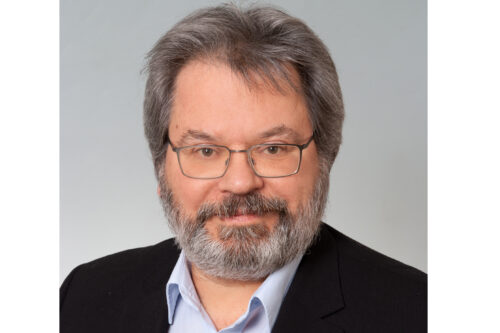
\includegraphics[scale=1.]{Figures/Schoeberl.jpg}
				\begin{center}
					\qquad\small Joachim Sc\"{o}berl
				\end{center}
			\end{figure}
			\vspace{0.3cm}
		\end{minipage}
	\end{frame}

	\begin{frame}[plain]
		$\newline$ 
		$\newline$ 
		\frametitle{PETSc}
		\petschead
		$\newline$
		$\newline$ 
		PETSc stands for Portable, Extensible Toolkit for Scientific Computation, is a library for the scalable (parallel) solution of scientific applications modeled by partial differential equations (PDEs).
		$\newline$
		\begin{minipage}{0.58\textwidth}
			\begin{itemize}
				\item[\color{oxfordblue}$\blacktriangleright$] \textbf{PETSc KSP} provides access to extremly efficent Krylov solvers.
				\item[\color{oxfordblue}$\blacktriangleright$] \textbf{PETSc SNES} provides access to extremly efficent non-linear solvers, with line-searching and trust region capabilities.
			\end{itemize}
		\end{minipage}
		\qquad
		\begin{minipage}{0.3\textwidth}
			\begin{figure}
				\centering
				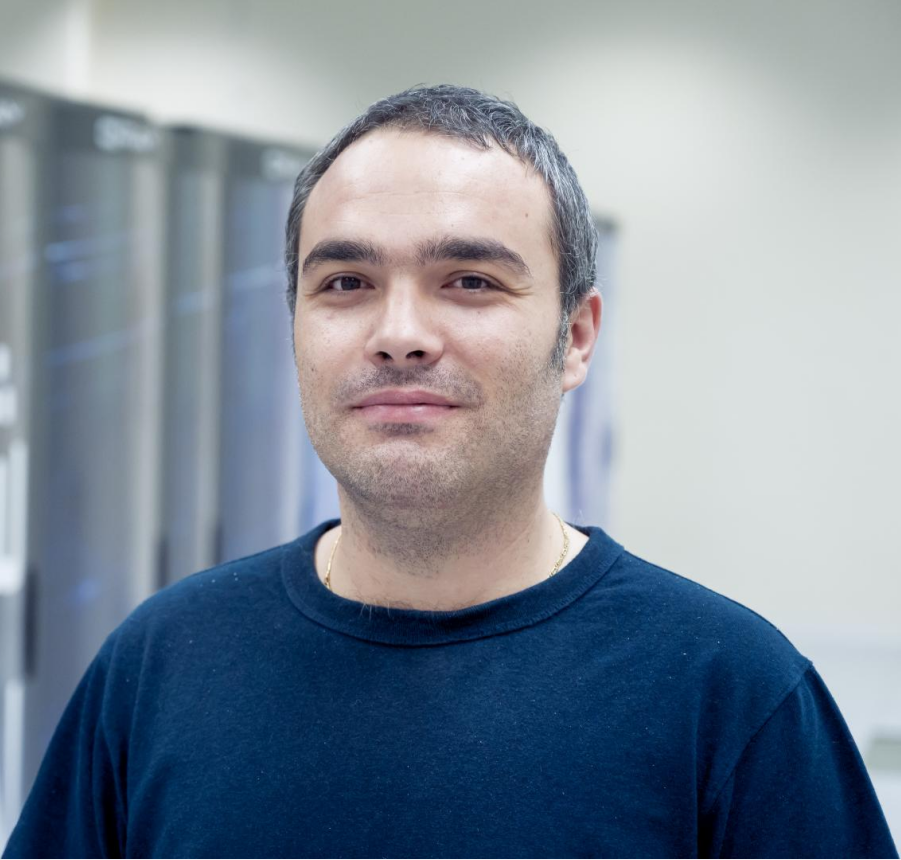
\includegraphics[scale=0.15]{Figures/Zampini.png}
				\begin{center}
					\;\;\small Stefano Zampini
				\end{center}
			\end{figure}
		\end{minipage}
		\vspace{3cm}
	\end{frame}
	\begin{frame}
		\frametitle{ngsPETSc -- NETGEN/NGSolve}
		$\newline$
		\textbf{ngsPETSc} is an interface between NETGEN/NGSolve and \textbf{PETSc}. In particular, \textbf{ngsPETSc} provides new capabilities to \textbf{NETGEN}/\textbf{NGSolve} such as:
		$\newline$
		\begin{itemize}
			\item[\color{oxfordblue}$\blacktriangleright$] Access to all linear solver capabilities of \textbf{KSP}.
			\item[\color{oxfordblue}$\blacktriangleright$] Access to all preconditioning capabilities of \textbf{PC}.
			\item[\color{oxfordblue}$\blacktriangleright$] Access to all non-linear solver capabilities of \textbf{SNES}.
			\item[\color{oxfordblue}$\blacktriangleright$] Access to all mesh refinement capabilities of \textbf{DMPLEX}.
		\end{itemize}
	\end{frame}
	\begin{frame}[plain]
		$\newline$ 
		\petschead
		\frametitle{PETSc DMPlex}
		$\newline$ 
		$\newline$
		\begin{minipage}{0.58\textwidth}
			\textbf{PETSc DMPlex} handles unstructured grids using the generic \textbf{PETSc} interface for hierarchy and multi-physics. 
			$\newline$
			\begin{itemize}
				\item[\color{oxfordblue}$\blacktriangleright$] \textbf{PETSc DMPlex} provides a wide variety of primitive mesh operations such as: \textit{meet}, \textit{clousre}, \textit{cone}, etc
				\item[\color{oxfordblue}$\blacktriangleright$] \textbf{PETSc DMPlex} provides a wide variety of mesh refinement operations such as: \textit{unifrom refinement}, \textit{Alfeld refinement}, \textit{box refinement}, etc
			\end{itemize}
		\end{minipage}
		\qquad
		\begin{minipage}{0.33\textwidth}
			\begin{figure}
				\centering
				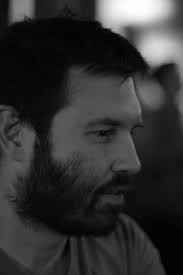
\includegraphics[scale=0.5]{Figures/Kneply.jpeg}
				\begin{center}
					\hspace{0.5cm}\small Matthew G.~Knepley
				\end{center}
			\end{figure}
		\end{minipage}
	\end{frame}
	\begin{frame}[plain]
		\firedrakehead
		$\newline$
		$\newline$
		\textbf{Firedrake} is an automated system for the solution of partial differential equations using the finite element method (FEM).
		$\newline$
		$\newline$
		\begin{minipage}{0.58\textwidth}
			\begin{itemize}
				\item[\color{oxfordblue}$\blacktriangleright$] Variational formulation can be easily defined using the \textbf{UFL} language.
				\item[\color{oxfordblue}$\blacktriangleright$] Wide class of finite elements are available, including $H(div)$, $H(curl)$, $H^1$ and $H^2$.
				\item[\color{oxfordblue}$\blacktriangleright$] Provides access to \textbf{PETSc} linear solvers and non-linear solvers.
			\end{itemize}
		\end{minipage}
		\qquad
		\begin{minipage}{0.3\textwidth}
			\begin{figure}
				\centering
				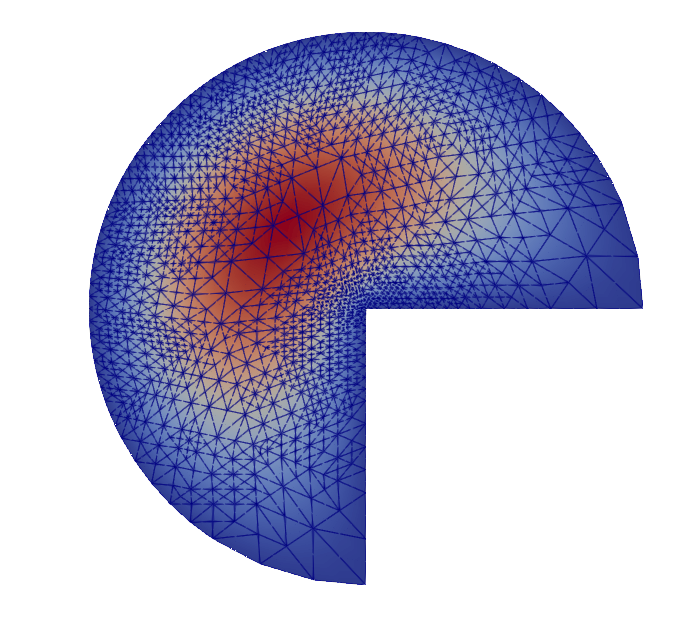
\includegraphics[scale=0.2]{Figures/Pacman.png}
			\end{figure}
			\vspace{0.3cm}
		\end{minipage}
	\end{frame}
	\begin{frame}
		\frametitle{ngsPETSc -- Firedrake}
		$\newline$
		\textbf{ngsPETSc} provides new capabilities to \textbf{Firedrake} such as:
		$\newline$
		\begin{itemize}
			\item[\color{oxfordblue}$\blacktriangleright$] Access to all Netgen generated linear meshes and high order meshes.
			\item[\color{oxfordblue}$\blacktriangleright$] Splits for macro elements, such as Alfeld splits and Powell-Sabin splits (even on curved geometries).
			\item[\color{oxfordblue}$\blacktriangleright$] Adaptive mesh refinement capabilities, that conform to the geometry.
			\item[\color{oxfordblue}$\blacktriangleright$] High order meshes hierarchy for multigrid solvers.
		\end{itemize}
	\end{frame}
	\begin{frame}{Examples -- Opencascade via NETGEN}
		\lstinputlisting[language=python,firstline=4,lastline=14]{Examples/occ.py}
	\end{frame}
	\begin{frame}{Examples -- Opencascade via NETGEN}
		$\newline$
		\lstinputlisting[language=python,firstline=15,lastline=17]{Examples/occ.py}
	\begin{figure}
			\centering
			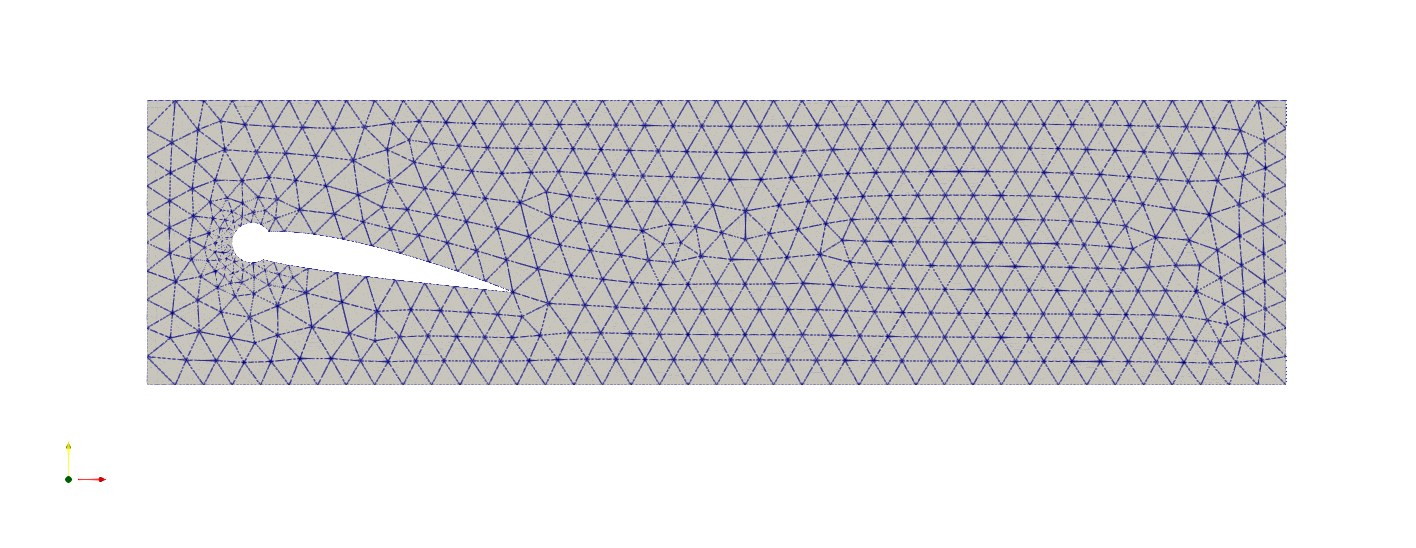
\includegraphics[scale=0.2]{Figures/nacaMesh.png}
		\end{figure}	
	\end{frame}
	\begin{frame}{Stokes flow -- Weak formulation}
		$\newline$
		Find $(\vec{u},p) \in V \times Q$ such that
		\begin{align*}
			\int_{\Omega} \nabla \vec{u} : \nabla \vec{v} - \int_{\Omega} p \nabla \cdot \vec{v} &= \int_{\Omega} \vec{f} \cdot \vec{v} \quad &\forall \vec{v} \in V \\
			\int_{\Omega} q \nabla \cdot \vec{u} &= 0 \quad &\forall q \in Q
		\end{align*}
		where $V$ and $Q$ are the velocity and pressure spaces respectively, i.e. $V = H^1_0(\Omega)^2$ and $Q = L^2_0(\Omega)$.
	\end{frame}
	\begin{frame}
		\frametitle{Stokes flow -- Inf-sup condition}
		$\newline$
		$\newline$
		We can also look for a discrete solution, i.e. find $(\vec{u}_h,p_h) \in V_h \times Q_h$ such that	
		\begin{minipage}{0.75\textwidth}
			\begin{gather}
				\nu\int_{\Omega} \nabla \vec{u} : \nabla \vec{v} - \int_{\Omega} p \nabla \cdot \vec{v} = \int_{\Omega} \vec{f} \cdot \vec{v}\\
				\int_{\Omega} q \nabla \cdot \vec{u} = 0
			\end{gather}
		for all $(\vec{v},q) \in V_h \times Q_h$.
		\begin{equation}
			\underset{q\in Q_h}{\inf} \underset{\vec{v}\in V_h}{\sup} \frac{\int_{\Omega} q \nabla \cdot \vec{v}}{\norm{q}_{L^2} \norm{\vec{v}}_{H^1}} \geq \beta > 0	
		\end{equation}
		\end{minipage}
		\begin{minipage}{0.2\textwidth}
			\begin{figure}
				\centering
				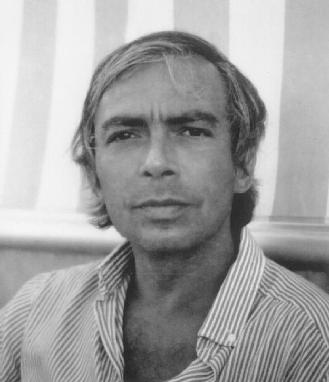
\includegraphics[scale=0.2]{Figures/Brezzi.jpg}
				\begin{center}
					\small Franco Brezzi
				\end{center}
			\end{figure}
		\end{minipage}
	\end{frame}
	\begin{frame}
		\frametitle{Stokes flow -- UFL}
		$\newline$
		\lstinputlisting[language=python,firstline=27,lastline=31]{Examples/scottVogelius.py}
	\end{frame}
	\begin{frame}
		\frametitle{Stokes flow -- Scott--Vogelius element}
		$\newline$
		$\newline$
		We can use the Scott--Vogelius pair, which is a mixed finite element of order $k$ for the velocity and order $k-1$ for the pressure.
		Such an element is inf-sup stable for $k \geq 2$, under certain assumptions on the mesh. Such pair is \textbf{divergence-free}.
		\begin{minipage}{0.75\textwidth}
			$\newline$	
			When $k=2$ we need \textbf{Alfeld splits}.
			\lstinputlisting[language=python,firstline=17,lastline=19]{Examples/scottVogelius.py}
			\lstinputlisting[language=python,firstline=24,lastline=26]{Examples/scottVogelius.py}
		\end{minipage}
		\begin{minipage}{0.2\textwidth}
			\begin{figure}
				\centering
				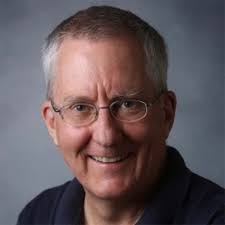
\includegraphics[scale=0.3]{Figures/Scott.jpeg}
				\begin{center}
					\small Ridgway Scott
				\end{center}
			\end{figure}
		\end{minipage}
	\end{frame}
	\begin{frame}
		\frametitle{Stokes flow -- Scott--Vogelius}
		$\newline$
		\lstinputlisting[language=python,firstline=38,lastline=41]{Examples/scottVogelius.py}
		\vspace{-1cm}
		\begin{figure}
			\centering
			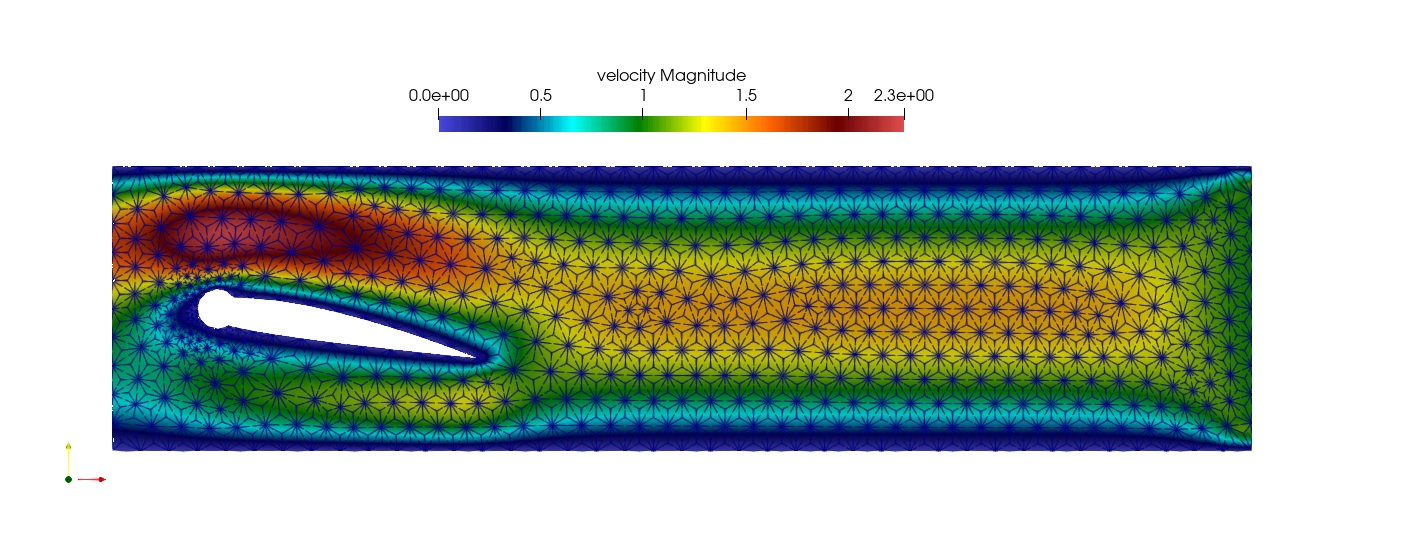
\includegraphics[scale=0.2]{Figures/scottVogelius.png}
		\end{figure}
	\end{frame}
	\begin{frame}
		\frametitle{Stokes flow -- Hood--Taylor element}
		$\newline$
		$\newline$
		Another element pair we will use is the Hood--Taylor pair, which has \textbf{no restrictions} on the mesh in two dimensions.
		$\newline$
		$\newline$
		\begin{minipage}{0.8\textwidth}
			\lstinputlisting[language=python,firstline=24,lastline=26]{Examples/hoodTaylor.py}
			\textbf{We lose the point-wise divergence-free property!}
			This is not an issue because the same would happen for Scott-Vogelius on curved meshes.
		\end{minipage}
		\begin{minipage}{0.18\textwidth}
			\begin{figure}
				\centering
				\qquad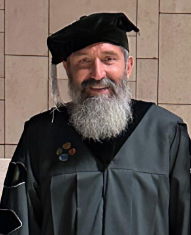
\includegraphics[scale=0.4]{Figures/Boffi.png}
				\begin{center}
					\small Daniele Boffi
				\end{center}
			\end{figure}
		\end{minipage}
	\end{frame}
	\begin{frame}{Fieldsplit Schur preconditioner}
		$\newline$
		$\newline$
		The previous set of equations can be written in matrix form as
		\vspace{-0.3cm}
		\begin{equation}
			\begin{bmatrix}
				A & B^T \\
				B & 0
			\end{bmatrix}
			\begin{bmatrix}\vec{u} \\p\end{bmatrix}=\begin{bmatrix}\vec{f} \\0\end{bmatrix}
		\end{equation}
		We choose as preconditioner the \textbf{fieldsplit Schur preconditioner}, i.e.
		\vspace{-0.3cm}
		\begin{equation}
			\begin{bmatrix}
				I & -\hat{A}^{-1} B^T\\
				0 & I
			\end{bmatrix}
			\begin{bmatrix}
				\hat{A}^{-1}& 0\\
				0 & \hat{S}^{-1}
			\end{bmatrix}
			\begin{bmatrix}
				I & 0\\
				-B\hat{A}^{-1} & I
			\end{bmatrix}
		\end{equation}
		where $S$ is the \textbf{Schur complement}, i.e. $S = -BA^{-1}B^T$.
		\lstinputlisting[language=python, firstline=18, lastline=21]{Examples/solvers.py}
	\end{frame}
	\begin{frame}
		\frametitle{Fieldsplit Schur preconditioner -- Mass matrix}
		$\newline$
		$\newline$
		Thanks to the inf-sup condition we can prove that the Schur complement is spectrally equivalent to the mass matrix, hence we can use as preconditioner:
		\begin{minipage}{0.7\textwidth}
			\vspace{-0.35cm}
			\begin{equation}
				\begin{bmatrix}
					I & -\hat{A}^{-1} B^T\\
					0 & I
				\end{bmatrix}
				\begin{bmatrix}
					\hat{A}^{-1}& 0\\
					0 & -\nu \hat{M}^{-1}
				\end{bmatrix}
				\begin{bmatrix}
					I & 0\\
					-B\hat{A}^{-1} & I
				\end{bmatrix}
			\end{equation}
			where $M$ is the mass matrix.
			\lstinputlisting[language=python,firstline=43,lastline=47]{Examples/multigrid.py}
		\end{minipage}
		\begin{minipage}{0.28\textwidth}
			\begin{figure}
				\centering
				\qquad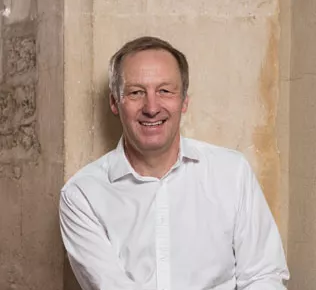
\includegraphics[scale=0.35]{Figures/Wathen.png}
				\begin{center}
					\small Andrew Wathen
				\end{center}
			\end{figure}
		\end{minipage}
	\end{frame}
	\begin{frame}{Multigrid on curved meshes}
		$\newline$
		ngsPETSc allows us to create a hierarchy of curved meshes for multigrid solvers.
		\lstinputlisting[language=python,firstline=19,lastline=21]{Examples/multigrid.py}
		We can than use a multigrid solver to compute $\hat{A}^{-1}$:
		\lstinputlisting[language=python,firstline=18,lastline=23]{Examples/solvers.py}
	\end{frame}
	\begin{frame}{Monolithic multigrid on curved meshes -- Coarse mesh}
		$\newline$
		We can also a monolithic multigrid solver for the Schur complement:
		\lstinputlisting[language=python,firstline=30,lastline=38]{Examples/solvers.py}
	\end{frame}
	\begin{frame}{Monolithic multigrid on curved meshes -- Fine mesh}
		$\newline$
		\lstinputlisting[language=python,firstline=43,lastline=53]{Examples/solvers.py}
	\end{frame}
	\begin{frame}{Navier-Stokes flow}
		A more interesting example is the Navier-Stokes flow, which is a non-linear problem.
		In particular, we will consider the problem of finding $(\vec{u},p) \in H^1(\Omega)^2\times L^2_0(\Omega)$ such that
		\begin{align*}
			\int_\Omega \partial_t \vec{u} \cdot \vec{v} + \int_\Omega(\nabla \vec{u})\vec{u}\cdot\vec{v}+\nu\int_{\Omega} \nabla \vec{u} : \nabla \vec{v} - \int_{\Omega} p \nabla \cdot \vec{v} &= \int_{\Omega} \vec{f} \cdot \vec{v}\\
			\int_{\Omega} q \nabla \cdot \vec{u} &= 0
		\end{align*}
		for all $(\vec{v},q) \in H^1(\Omega)^2\times L^2_0(\Omega)$.
	\end{frame}
	\begin{frame}{Navier-Stokes flow -- Augmented Lagrangian}
		$\newline$
		We consider an augmented Lagrangian formulation for the discrete problem, i.e. find $(\vec{u}_h,p_h) \in V_h \times Q_h$ such that
		\begin{align*}
			(\partial_t\vec{u},\vec{v})_0 + (\nabla \vec{u}\vec{u},\vec{v})_0 &+ \nu(\nabla \vec{u},\nabla \vec{v})_0 \\
			 & - (p,\nabla \cdot \vec{v})_0 + \frac{\gamma}{2}(\nabla \cdot \vec{u},\nabla \cdot \vec{v})_0 &= (\vec{f},\vec{v})_0\\
		\end{align*}
		and verifying the weak divergence free constraint $(\nabla \cdot \vec{u},q)_0 = 0$, for all $(\vec{v},q) \in V_h \times Q_h$.
	\end{frame}
	\begin{frame}
		\frametitle{Navier-Stokes flow -- Fieldsplit Schour preconditioner}
		$\newline$
		$\newline$
		The linearized version of the Navier-Stokes equations can be written in matrix form as 
		\vspace{-0.3cm}
		\begin{equation}
			\begin{bmatrix}
				A+\gamma B^TWB& B^T \\
				B & 0
			\end{bmatrix}
			\begin{bmatrix}\vec{u} \\p\end{bmatrix}=\begin{bmatrix}\vec{f} \\0\end{bmatrix}
		\end{equation}
		We choose as preconditioner the \textbf{fieldsplit Schur preconditioner}, i.e.
		\vspace{-0.3cm}
		\begin{equation}
			\begin{bmatrix}
				I & -\hat{A}_\gamma^{-1} B^T\\
				0 & I
			\end{bmatrix}
			\begin{bmatrix}
				\hat{A}_\gamma^{-1}& 0\\
				0 & \hat{S}_\gamma^{-1}
			\end{bmatrix}
			\begin{bmatrix}
				I & 0\\
				-BA_\gamma^{-1} & I
			\end{bmatrix}
		\end{equation}
		\begin{equation}
			A_\gamma = A+\gamma B^TWB 	\qquad  S_\gamma = -BA_\gamma^{-1}B^T.
		\end{equation}
		In this case, we notice that independently of the Reynolds numbers $S_\gamma\sim - (\nu+\gamma)^{-1} M$.
	\end{frame}
	\begin{frame}{Navier-Stokes flow -- Augmented Lagrangian}
		$\newline$
		\begin{itemize}
			\item [\color{oxfordblue}$\blacktriangleright$] The augmented Lagrangian term helps enforce the divergence-free constraint, and makes the scheme pressure robuts.
			\item [\color{oxfordblue}$\blacktriangleright$] We can use as preconditioner
			\begin{equation}
				\begin{bmatrix}
					I & -\hat{A}_\gamma^{-1} B^T\\
					0 & I
				\end{bmatrix}
				\begin{bmatrix}
					\hat{A}_\gamma^{-1}& 0\\
					0 & -(\nu+\gamma)M^{-1}
				\end{bmatrix}
				\begin{bmatrix}
					I & 0\\
					-BA_\gamma^{-1} & I
				\end{bmatrix}
			\end{equation}
			\item[\color{oxfordblue}$\blacktriangleright$] How do we compute $\hat{A}_\gamma^{-1}$ efficiently ? Can we adopt a multigrid approach ?
		\end{itemize}
	\end{frame}
	\begin{frame}
		\frametitle{Subspace correction methods for nearly singular
problems}
		$\newline$
		$\newline$
		To compute $\hat{A}_\gamma^{-1}$ we can use a subspace correction method.
		We decompose the space $V_h$ as follows:
		\vspace{-0.3cm}
		\begin{equation}
			V_h = \sum_{i=1} V_i.
		\end{equation}
		We consider a coarse space $V_H$ and the projection and injection operators:
		\vspace{-0.3cm}
		\begin{equation}
			P_H : V_H \rightarrow V_h, \qquad I : V_h \rightarrow V_i.
		\end{equation}
		We then consider as smoother the additive Schwarz preconditioner defined as:
		\begin{equation}
			\hat{A}_\gamma^{-1} = P_H A_{\gamma,H}^{-1} P_H^T + \sum_{i=1} I_i A_{\gamma,i}^{-1} I_i^T.
		\end{equation}
	\end{frame}
	\begin{frame}
		\frametitle{Subspace correction methods for nearly singular
problems}
		$\newline$
		\begin{block}{Robust relaxetion}
			We need the discrete kernel,
			\vspace{-0.3cm}
			\begin{equation}
				\mathbb{K}_h =  \{\vec{v} \in V_h : B\vec{v} = 0\},
			\end{equation}
			to decompose in a \textbf{stable} way as follows:
			\vspace{-0.3cm}
			\begin{equation}
				\mathbb{K}_h = \sum_{i=1} \mathbb{K}_h\cap V_i.
			\end{equation}
		\end{block}
	\end{frame}
	\begin{frame}[fragile]
		\frametitle{Robust relaxation -- Hood--Taylor}
		\begin{equation*}
			\begin{tikzcd}[row sep=huge]
			0 \arrow[r,""] & \Big[H^2(\Omega)\Big]^2 \arrow[r,"\curl"] \arrow[d]& \Big[H^1_0(\Omega)\Big]^2 \arrow[r,"\div"] \arrow[d]& L^2_0(\Omega) \arrow[r,""]\arrow[d] & 0\\
			0 \arrow[r,""] & \Big[\mathbb{P}^4(\mathcal{T}_h)\Big]^2 \arrow[r,"\curl"] & \Big[\mathbb{P}^3(\mathcal{T}_h)\Big]^2 \arrow[r,"\div"] & \mathbb{P}^2_{disc}(\mathcal{T}_h) \arrow[r,""] & 0\\
			\end{tikzcd}
		\end{equation*}
		\vspace{-2cm}
		\begin{figure}[h]
			\centering
			\hspace{1cm}\scalebox{0.45}{\tikzfig{Figures/DoF}}
		\end{figure}
	\end{frame}
	\begin{frame}
		\frametitle{Robust prolongation -- Hood--Taylor}
		$\newline$
		\begin{block}{Robust relaxetion}
			If the space pair $(V_h,Q_h)$ is inf-sup stable and the mesh we have a robust prolongation operator defined by:
			\begin{equation}
				\tilde P_H \vec{u}_H - \tilde{\vec{u}}_h = \vec{u}_H-\tilde{\vec{u}}_h,
			\end{equation}
			where
			\begin{equation}
				a_{\gamma}(\tilde{\vec{u}}_h,\tilde{\vec{v}}_h) = \gamma(\nabla \cdot \tilde{\vec{u}}_h,\nabla \cdot \tilde{\vec{v}}_h)_{\pi_{Q_h}\pi{Q_h}^T} \quad \forall \tilde{\vec{v}}_h \in \tilde{V}_h,
			\end{equation}
			where $\pi_{Q_h}$ is the $L^2$ projection onto $Q_h$ and $\tilde{V}_h$ is the space of discrete velocity vanishing at the boundary of the coarse cells.
		\end{block}
	\end{frame}
	\begin{frame}
		\frametitle{Numerical Simulation}
		\begin{figure}
			\centering
			\scalebox{0.2}{\animategraphics[loop,autoplay]{12}{Figures/NS/Velocity.}{0000}{0158}}
		\end{figure}
	\end{frame}
\end{document}
